% !TeX encoding = UTF-8
% !TeX program = pdflatex

\documentclass[Lau,binding=0.6cm,oneside]{sapthesis}

\usepackage{microtype}
\usepackage[english]{babel}
\usepackage[utf8]{inputenx}
\usepackage[backend=biber,sorting=none]{biblatex}
\usepackage[titletoc]{appendix}
\usepackage{amsmath}
\usepackage[ruled,longend]{algorithm2e}
\usepackage{amssymb}
\usepackage{amsthm}
\usepackage{mathrsfs}
\usepackage{graphicx}
\usepackage{hyperref}
\usepackage{float}
\usepackage{minted}
\usepackage{color}
\usepackage{afterpage}
\usepackage[most]{tcolorbox}
\usepackage{csquotes}
\usepackage{xcolor}
\usepackage{colortbl}
\usepackage{hhline}
\usepackage[symbol]{footmisc}

\graphicspath{ {./images/} }

\hypersetup{pdftitle={Substitution ciphers: cryptanalysis and other attacking techniques},pdfauthor={Daniele Cappuccio}}

\addbibresource{bibliography.bib}

% Remove in a normal thesis
\usepackage{lipsum}
\usepackage{curve2e}
\definecolor{gray}{gray}{0.4}
\newcommand{\bs}{\textbackslash}

% [DC] This command lets us use symbols instead of numbers to mark footnotes
\renewcommand{\thefootnote}{\fnsymbol{footnote}}

% Commands for the titlepage
\title{Substitution ciphers: cryptanalysis \\and other attacking techniques}
\author{Daniele Cappuccio}
\IDnumber{1703987}
\course{Ingegneria Informatica}
\courseorganizer{Facoltà di Ingegneria dell'informazione, informatica e statistica}
\AcademicYear{2017/2018}
\copyyear{2018}
\advisor{Prof. Fabrizio d'Amore}
\authoremail{daniele97bsk@gmail.com}

% \examdate{01 January 2018}
% \examiner{Prof. Nome Cognome}
% \examiner{Prof. Nome Cognome}
\versiondate{\today}

\newtheorem{theorem}{Theorem}


\begin{document}

\frontmatter

\maketitle

\dedication{Dedicated to\\Alan Turing}

\begin{abstract}\phantomsection\addcontentsline{toc}{chapter}{Abstract}

The thesis is based upon classical cryptography, in particular substitution ciphers, with an emphasis put on both the strength and complexity of the various encryption and decryption schemes, and the well-known breaking techniques a potential attacker can employ.

The last chapter covers a real-world case, the Zodiac ciphers, a series of broken and unbroken ciphertexts left by a serial killer in the late `60s. We focus on designing and implementing an efficient solution to one of these ciphers, known as the \textsf{Zodiac-408}.

\end{abstract}

\begin{acknowledgments}\phantomsection\addcontentsline{toc}{chapter}{Acknowledgments}

First, I would like to thank my parents, my family, my girlfriend and my closest friends for providing me with unfailing support and continuous encouragement throughout my years of study and through the process of writing this thesis. This accomplishment would not have been possible without them.

I would also like to acknowledge my fellow students for making tough lessons less tiring, and for offering me food for thought when studying together.

Finally, I express my sincere gratitude to my advisor Prof.\ D'Amore for his patience, guidance and insightful comments.
\end{acknowledgments}

\tableofcontents

\mainmatter

\chapter{Introduction}
In a world governed by the circulation of information in every possible form and in any possible way, security has become a major problem. \textbf{Information security} (or InfoSec), which is a practice of preventing the disruption, modification, or simply unauthorized access of info, arose drastically in the last few decades, especially after the digital era began. However, since the early days of communication, diplomats and military commanders understood that it was necessary to provide some mechanisms to protect the confidentiality of correspondence and to have some means of detecting tampering.

\section{Information Security's key concepts}
Information security's primary focus is the balanced protection of the \textit{confidentiality}, \textit{integrity} and \textit{availability} of data (also known as the \textbf{CIA triad}) while maintaining a focus on efficient policy implementation, all without hampering productivity. This model is often designed to guide policies for InfoSec within an organization. In this context, confidentiality is a set of rules that limits access to information, integrity is the assurance that the information is trustworthy and accurate, and availability is a guarantee of reliable access to the information by authorized people.

\subsection{Confidentiality}
Confidentiality is roughly equivalent to privacy. Measures undertaken to ensure confidentiality are designed to prevent sensitive information \textbf{reaching the wrong people}, while making sure that the right people can in fact get it: access must be restricted to those authorized to handle the given data. It is common, as well, for data to be categorized according to the amount and type of damage that could be done when leaked to unintended people\supercite{confidentiality}.\\\\
Data encryption is a common method of ensuring confidentiality: the main aim of every cryptographic scheme is that of being sure that data cannot be accessed by unapproved people.

\subsection{Integrity}
Data integrity means maintaining and assuring the accuracy and completeness of data over its entire lifecycle: this means that data cannot be modified in an unauthorized or undetected manner\supercite{integrity}. Information security systems typically provide message integrity in addition to data confidentiality.

\subsection{Availability}
For any information system to serve its purpose, the information must be available when it is needed. In the realm of information security, availability can often be viewed as one of the most important parts of a successful information security program: by ensuring availability, for instance, an organization is able to perform to the standards that an organizations stake-holders expect.

\section{The role of cryptography}
\textbf{Cryptography} (or \textbf{cryptology}) developed a major role in ensuring confidentiality: since the first known forms of cryptography, the biggest concern was that of keeping information private and/or secret. Nowadays, whether it be passwords sent during a log on process, or storing confidential medical records in a database, encryption can assure that only the parties that have access to the appropriate key will get access to the effective data.\\\\
Various types of cryptographic systems exist that have different strenghts and weaknesses. Typically, they are divided into two main classes: those that are strong, but slow to run, and those that are quick, but less secure. Most often a combination of the two approaches is used (e.g.: modern SSL communication), whereby we establish the connection with a secure algorithm, and then if successful, encrypt the actual transmission with the weaker, but much faster algorithm.

\subsection{Symmetric cryptography}
Symmetric cryptography is the most traditional form of cryptography. In a symmetric cryptosystem, the involved parties share a common secret (password, pass phrase, or key). Data is encrypted and decrypted using the same key\supercite{symmetric}. These algorithms tend to be comparatively fast, but they cannot be used unless the involved parties have already exchanged their keys. Any party possessing a specific key can create encrypted messages using that key as well as decrypt any messages encrypted with the key.\\\\
In systems involving a number of users who need to set up independently, secure communication channels symmetric cryptosystems can have practical limitations due to the requirement to securely distribute and manage large numbers of keys.

\subsection{Asymmetric cryptography}
Asymmetric algorithms, on the other hand, use two different keys, one to encrypt the data, and the other one to decrypt. These independent keys are generated together. One is labeled the \textit{public key} and is distributed freely; the other is labeled the \textit{private key} and must be kept secret\supercite{asymmetric}.\\\\
The most common usage of asymmetric cryptography is to send messages with a guarantee of confidentiality. If user A wants to send a message to user B, A would get access to user B's publicly-available public key. The message is then encrypted with this key and sent to user B. Because of the cryptosystem's property that messages encoded with the public key of B can only be decrypted with user B's private key, only user B can clearly read the message.\\\\
Another usage scenario is one where user A wants to send user B a message and wants user B to have a guarantee that the message was sent by A. In order to accomplish this, A would encrypt the message with their private key. The message can then only be decrypted using A's public key. This guarantees that user A created the message because they are the only entity who had access to the private key required to create a message that can be decrypted by A's public key. This is essentially a digital signature guaranteeing that the message was created by user A.

\section{Classical ciphers}
Historically, the first examples of a cipher, i.e. a series of well-defined steps can be followed as a procedure in order to encrypt or decrypt a message, date back to the ancient Greeks, in particular a scytale transposition cipher used by the Spartan military. Since then, a plethora of different ciphers have been developed, with different scopes and various complexity. With the term classical cipher, we deal with all symmetric algorithms developed until the 1970s: these ciphers have now fallen, for the most part, into disuse. In contrast to modern cryptographic algorithms, most classical ciphers can be practically computed and solved by hand, although they are even simpler to break with modern computers.\\\\
Classical ciphers are often divided into two big groups: \textit{transposition ciphers}\footnote[1]{See Appendix A} and \textit{substitution ciphers}. The former group is a family of algorithms in which the letters of the message are kept unchanged, but their order is scrambled according to some well-defined scheme, for example a geometric design. The latter is a method of encrypting by which units of plaintext are replaced with ciphertext, according to a fixed system; the units may be single letters (the most common), pairs of letters, triplets of letters, and so forth.\\\\
In this thesis, we'll focus our attention on substitution ciphers: we'll deal with famous historical ones and later analyze some strong techniques that can be used to break them, with the help of software or simply by hand.

\chapter{Monoalphabetic ciphers}
The simplest form of substitution ciphers is the \textbf{monoalphabetic cipher}, which is also called simple substitution cipher: every letter of the alphabet is replaced separately, determining a so-called substitution alphabet. Common uses of the substitution alphabet consist in shifting (Caesar cipher) or reversing (Atbash cipher): more complex and scrambled alphabets are usually named \textit{mixed alphabets} or \textit{deranged alphabets}.\\\\

\begin{figure}[h]
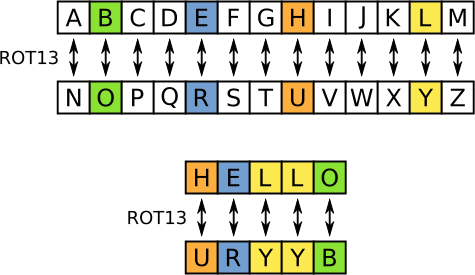
\includegraphics[scale=0.4]{rot13}
\captionsetup{justification=centering, margin=2cm}
\centering
\caption{\textsf{ROT13} is a type of Caesar cipher, in which every letter is `rotated' of 13 positions within the English alphabet.}
\centering
\end{figure}

\section{Keyword cipher}

A traditional way of creating new mixed alphabets follows: a keyword is written out, the repeated letters in it are removed, and at the end all the remaining letters in the alphabet use the standard order. Using this system, the keyword \textsf{helloworld} creates the following ciphertext alphabet:\\\\
	\textbf{\small{Plaintext alphabet}}: \par\colorbox{gray!12}{\small{\texttt{ABCDEFGHIJKLMNOPQRSTUVWXYZ}}}\\
	\textbf{\small{Ciphertext alphabet}}:	\par\colorbox{gray!12}{\small{\texttt{HELOWRDABCFGIJKMNPQSTUVXYZ}}}\\
\ \\
Trivially, the ciphertext is written out in blocks of fixed length, omitting punctuation and spaces; this is done to help avoid transmission errors and to disguise word boundaries from the plaintext. These blocks are called `groups'. When the telegraph was invented, five-letter groups was the common way of transmitting messages. In the frequent case the length of the message happens not to be divisible by five, it has to be padded at the end with `nulls', i.e. with any characters which result in nonsense when decrypted: in this way, the receiver can easily spot them and discard them. \\\\
However, a disadvantage of this scheme of derangement is that the last letters of the alphabet (which are mostly low frequency) tend to remain at the end. Although it is not often done, a more secure way of constructing a mixed alphabet is to perform columnar transpositions on the ordinary alphabet using the chosen keyword.\\\\
The ciphertext alphabet provided above encrypts \colorbox{gray!12}{\small{\texttt{LOREM IPSUM DOLOR}}}
into\\ \colorbox{gray!12}{\small{\texttt{GKPWI BMQTI OKGKP}}}.

\section{Caesar cipher}
The \textbf{Caesar cipher} is the first example of widely known encryption techniques based on monoalphabetic substitution. The method is named after Julius Caesar, who frequently used it in his private correspondence. \\\\
Fun fact, it was the first recorded use of this type of schemes, although other ciphers are known to have been used earlier.\\\\
Each letter in the plaintext is replaced by another letter which is some fixed number of positions down the alphabet. For instance, \textsf{D} shall be replaced by \textsf{A}, if we're using a left shift of 3.\\\\
Encryption and decryption can also be represented using modular arithmetic by first transforming the letters into numbers, according to the traditional scheme $A \rightarrow 0,\\ B \rightarrow 1, ... , Z \rightarrow 25$, like this:\\

\begin{equation}
E_{n}({x}) = (x + n) \ mod \ 26
\end{equation}

\begin{equation}
D_{n}({x}) = (x - n) \ mod \ 26
\end{equation}

\newpage

\begin{figure}[H]
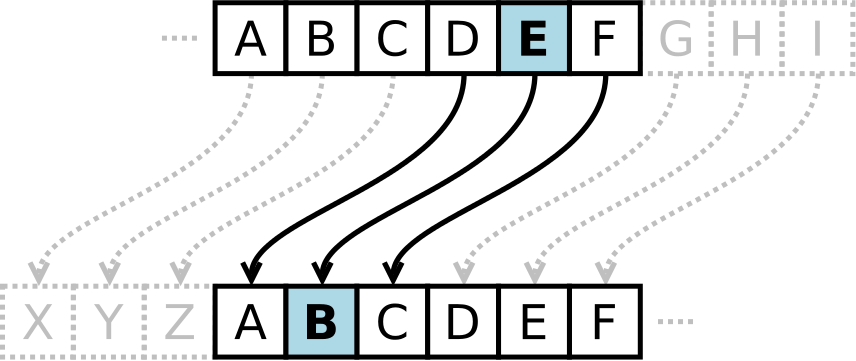
\includegraphics[scale=0.34]{caesar_cipher}
\centering
\caption{With a left shift of 3, the letter \textsf{E} is replaced by the letter \textsf{B}}
\centering
\end{figure}

\ \\
Nonetheless, the Caesar cipher can be easily broken, especially using a computer, and in modern practice it offers no communication security whatsoever; hence, the encryption step performed by this cipher is only incorporated as part of more complex schemes, such as the Vigenère cipher.

\section{Atbash cipher}
The \textbf{Atbash cipher} is another simple substitution cipher, which was originally used to encrypt the Hebrew alphabet, though it can be slightly changed for use with any known writing system with a standard collating order.\\\\
The cipher consists in mapping each letter of the alphabet to its reverse, in a way that the first letter becomes the last letter, the second letter becomes the second to last letter, and so on. For example, the Latin alphabet would work like this: \\

\begin{figure}[H]
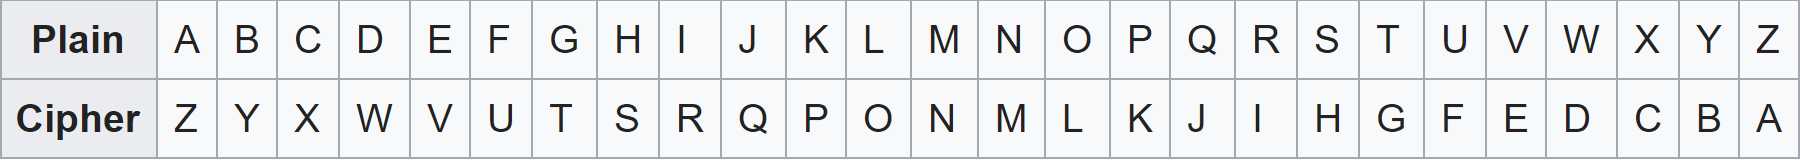
\includegraphics[scale=0.65]{atbash_cipher}
\centering
\caption{}
\centering
\end{figure}

\ \\
Several biblical verses are described as being examples of Atbash\supercite{atbash}.\\

\section{Pigpen cipher}
The \textbf{pigpen cipher} (alternately referred to as Napoleon cipher) is a geometric simple substitution cipher, which exchanges letters for symbols which are fragments of a grid.\\\\
The use of symbols instead of letters is no impediment to cryptanalysis, as this scheme is practically identical to other monoalphabetic substitution ones.\\\\

\begin{figure}[h]
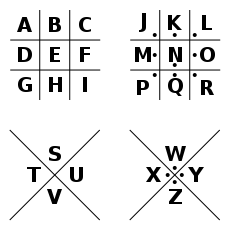
\includegraphics[scale=0.4]{pigpen}
\centering
\caption{An example of graphical symbols used in a pigpen cipher}
\centering
\end{figure}

Using the Pigpen cipher key described above, the message \textsf{X MARKS THE SPOT} is rendered in ciphertext as:\\\\

\begin{figure}[h]
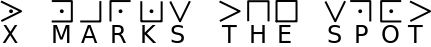
\includegraphics[scale=0.7]{xmarksthespot}
\centering
\caption{}
\centering
\end{figure}

\section{Affine cipher}
The \textbf{affine cipher} is another type of monoalphabetic substitution cipher, wherein each letter in an alphabet is first mapped to its numeric equivalent, then encrypted using a function, and lastly converted back to a letter. However, each letter encrypts to one other letter, meaning the cipher is essentially a standard substitution cipher with a rule governing which letter converts to which. As such, it has all the weaknesses of similar substitution ciphers\supercite{affine}.\\\\
In the affine cipher the letters of an alphabet of size $m$ are first mapped to the integers in the range $0 ... m-1$. Modular arithmetic is subsequently used to transform the integer into another integer that corresponds to a ciphertext letter.\\\\ The encryption function for a single letter is:

\begin{equation}
E{(x)} = (ax + b) \ mod \ m
\end{equation}

\ \\where modulus $m$ is the size of the alphabet and $a$ and $b$ are the key of the cipher. Obviously, the value $a$ must be chosen such that $a$ and $m$ are coprime; in fact, the decryption function is:

\begin{equation}
D{(x)} = a^{-1}(x-b)\ mod \ m
\end{equation}

\ \\and $a^{-1}$, which is the modular multiplicative inverse of $a$ modulo $m$ exists only if $GCD(a, m) = 1$.\\\\
To prove that the decryption function is the inverse of the encryption function:

\begin{equation}
\begin{split}
D{(E{(x)})} &= a^{-1}(E{(x)}-b)\ mod\ m\\
				&= a^{-1}(((ax + b) \ mod \ m) - b)\ mod\ m\\
				&= a^{-1}(ax + b - b) \ mod \ m\\
				&= a^{-1}ax \ mod \ m\\
				&= x \ mod \ m\\
\end{split}
\end{equation}
\ \\
For example, let's choose $a = 5$ and $b = 8$, with $m = 26$ since there are 26 characters in the alphabet being used. To encrypt the word \textsf{AFFINECIPHER} we just have to follow the mathematical rules and apply them to the values chosen above. \\\\We can fill out a table like this:\\\\

\begin{figure}[H]
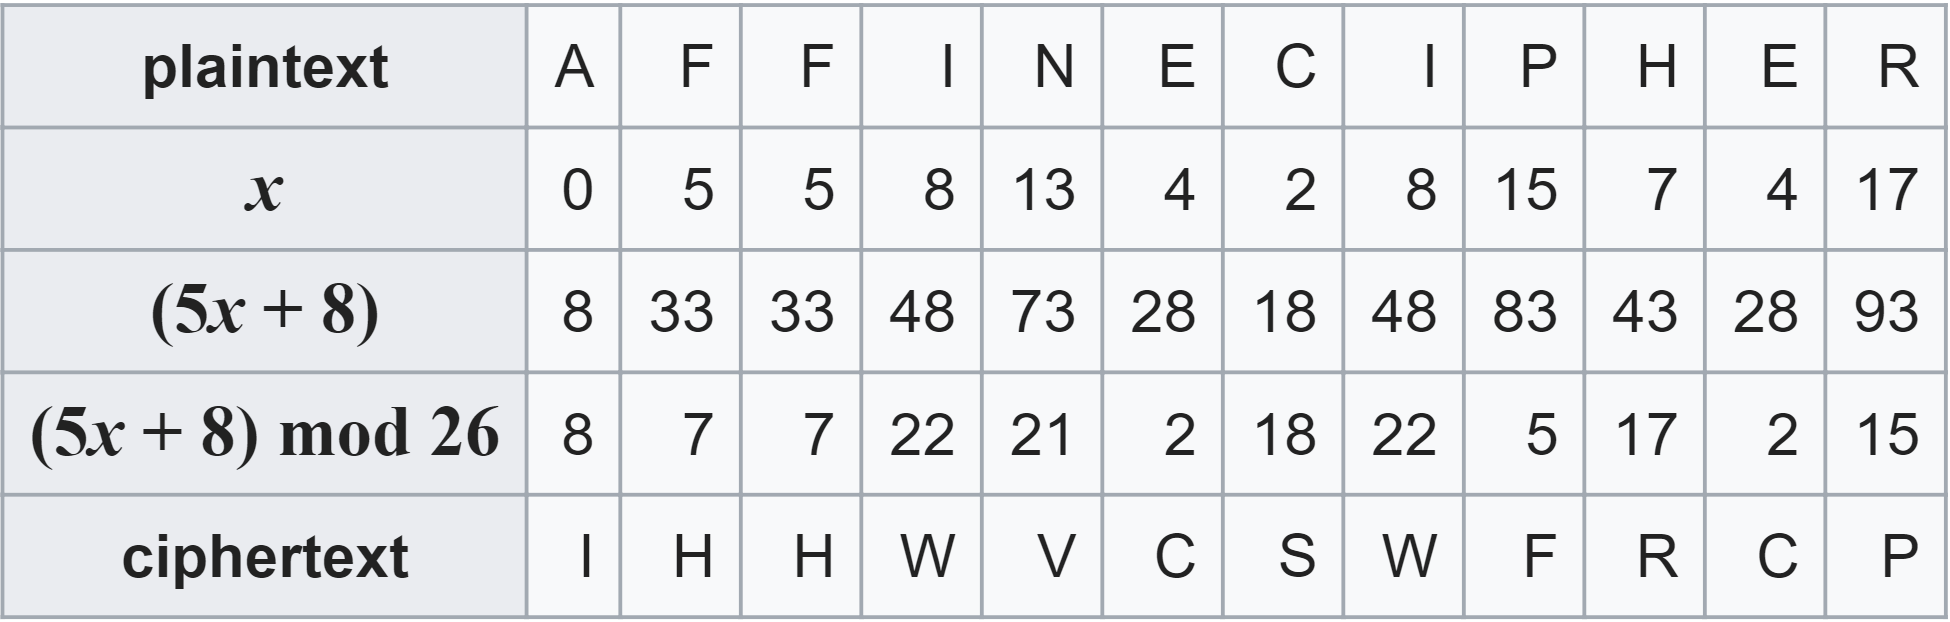
\includegraphics[scale=0.5]{affine_encrypt}
\captionsetup{justification=centering, margin=2cm}
\centering
\caption{The word \textsf{AFFINECIPHER} results in \texttt{IHHWVCSWFRCP} using an affine cipher with a = 5 and b = 8.}
\centering
\end{figure}
\ \\
When decrypting, we first have to compute $a^{-1}$, i.e.\ the multiplicative inverse, which is 21 in this case. The corresponding decryption function will be\\
\begin{equation}
D{(y)} = 21(y-8) \ mod \ 26
\end{equation}
\ \\
Once we have the decryption function, the final step will be that of using the table to convert numeric values back into letters.\\\\

\begin{figure}[H]
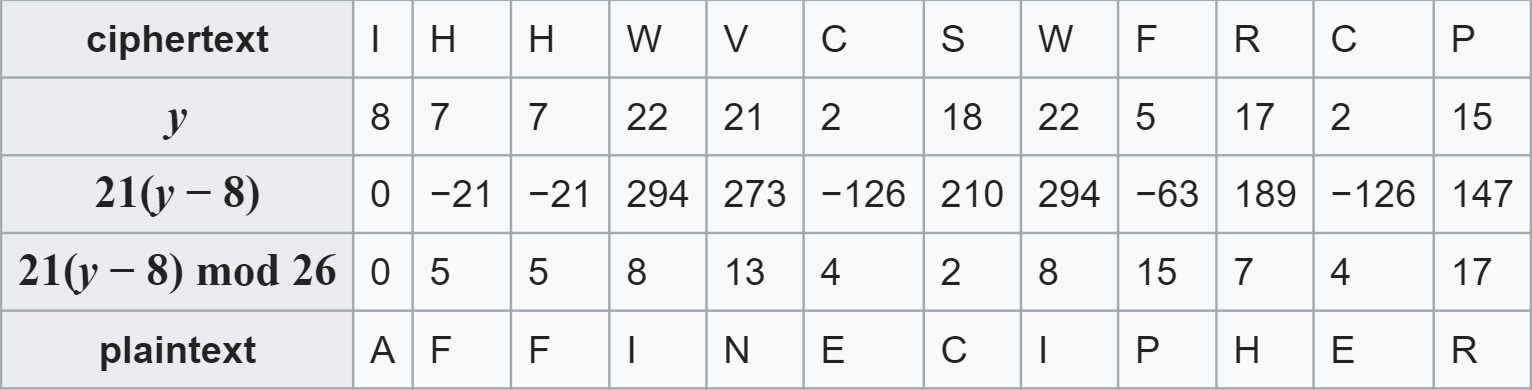
\includegraphics[scale=0.68]{affine_decrypt}
\centering
\caption{}
\centering
\end{figure}	

\subsection{Atbash cipher as a particular affine cipher}
The Atbash cipher can be seen as a special case of the affine cipher.\\\\
Under the standard affine convention, an alphabet of $m$ letters is mapped to the numbers $0,1, ..., m-1$. The Atbash cipher may then be enciphered and deciphered using the encryption function for an affine cipher, by setting $a=b=m-1$

\begin{equation}
E{(x)} = D{(E{(x)})} = ((m-1)x + (m-1)) \ mod \ m
\end{equation}
\ \\
which can be simplified to:

\begin{equation}
E{(x)} = (m-1)(x-1) \ mod \ m = -(x+1) \ mod \ m
\end{equation}

\ \\
Here follows an implementation of an affine cipher using the Python programming language, specifically the \textsf{Python 3.5} version (the \texttt{gcd} library function was introduced since this version).\\

\newmintedfile[pythonic]{python}{
	linenos = true,
	numberblanklines = true,
	frame=lines,
	framesep=2mm
}

\pythonic{code/affine_cipher.py}
\ \\
\section{Security for monoalphabetic substitution ciphers}
The number of possible keys is extraordinarily large (26!); nevertheless, this kind of ciphers can be easily broken. Provided the message is of moderate length, a cryptanalyst can deduce the probable meaning of every symbol by analyzing the frequency distribution of the ciphertext. This allows formation of partial words, which can be tentatively filled in, progressively expanding the solution.\\\\
In some cases, underlying words can also be determined from the pattern of their letters; for example, the words \textit{attract} and \textit{osseus} (and words with those two as the root) are the only common English words with the pattern \textsf{ABBCADB}. Many people solve such ciphers for recreation, as with cryptogram puzzles in the newspaper.\\\\
According to the unicity distance of English, 27.6 letters of ciphertext are required to crack a mixed alphabet simple substitution. In practice, typically about 50 letters are needed, although some messages can be broken with fewer if unusual patterns are found. In other cases, the plaintext can be contrived to have a nearly flat frequency distribution, and much longer plaintexts will then be required by the cryptanalyst.

\chapter{Polyalphabetic ciphers}
The first chapter discussed ciphers based on monoalphabetic substitution, which are the ones that encode data using only \textit{one} alphabet (hence the Greek root \textit{mono} meaning `one'). As we stated earlier, these are fairly easy to break, especially when the spaces between words are still there.\\\\
How can it be made harder to decrypt messages? Well, one way is to use \textbf{more than one} alphabet, switching between them systematically. This type of cipher is called a \textbf{polyalphabetic substitution cipher} (\textit{poly} is the Greek root for `many'); the main difference is that frequency analysis no longer works the same way to break these kind of ciphers.\\\\
The Vigenère cipher is probably the best-known example of a polyalphabetic cipher, though it is a simplified special case. The Enigma machine, which was used during World War Two, is more complex but it is still fundamentally a polyalphabetic substitution cipher.

\section{Alberti cipher}
The \textbf{Alberti cipher} is probably the first polyalphabetic cipher ever created (15th century), and it was the peak of cryptography at that time. Its inventor was Leon Battista Alberti, an Italian artist, architect, poet, linguist, philosopher (and obviously, cryptographer!).\\\\

\begin{figure}[H]
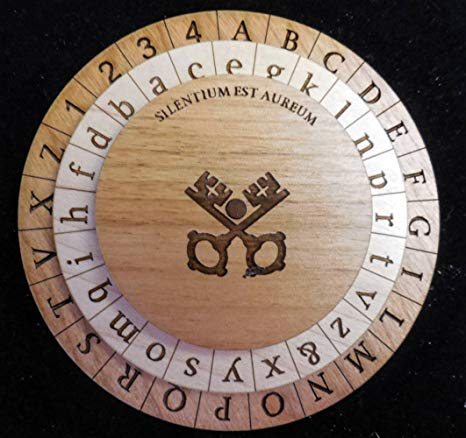
\includegraphics[scale=0.5]{alberti_cipher_disk}
\centering
\caption{A copy of the Alberti cipher disk.}
\centering
\end{figure}
\ \\
In his treatise \textit{De Cifris} Leon Battista Alberti described his \textbf{Cipher Disk}, which he called \textit{Formula}, as made up of two concentric disks, attached by a common pin, which can rotate one with respect to the other.\\\\
The larger one is called \textit{Stabilis} (meaning `stationary' or `fixed'), meanwhile the smaller one is called \textit{Mobilis} (meaning `movable'). The circumference of each disk is divided into 24 equal cells.\\\\
The outer ring contains one uppercase alphabet for plaintext and the inner ring has a lowercase mixed alphabet for ciphertext. The outer ring also includes the numbers 1 to 4 for the superencipherment of a codebook containing 336 phrases with assigned numerical values.\\\\
This is a very effective method of concealing the code-numbers, since their equivalents cannot be distinguished from the other garbled letters. The sliding of the alphabets is controlled by key letters included in the body of the cryptogram\supercite{alberti}.\\\\

\section{Trithemius cipher}
The \textbf{Trithemius cipher} was invented by Johannes Trithemius, who described it in his book \textit{Polygraphia}, which is credited with being the first published work on cryptology\supercite{trithemius}.\\\\
Trithemius used a \textbf{tabula recta}, which is a square table of alphabets, each row of which is made by shifting the previous one to the left. In this way, he defined a polyalphabetic cipher that is somehow equivalent to Alberti's cipher disk except that the alphabets are not mixed.\\\\

\begin{figure}[H]
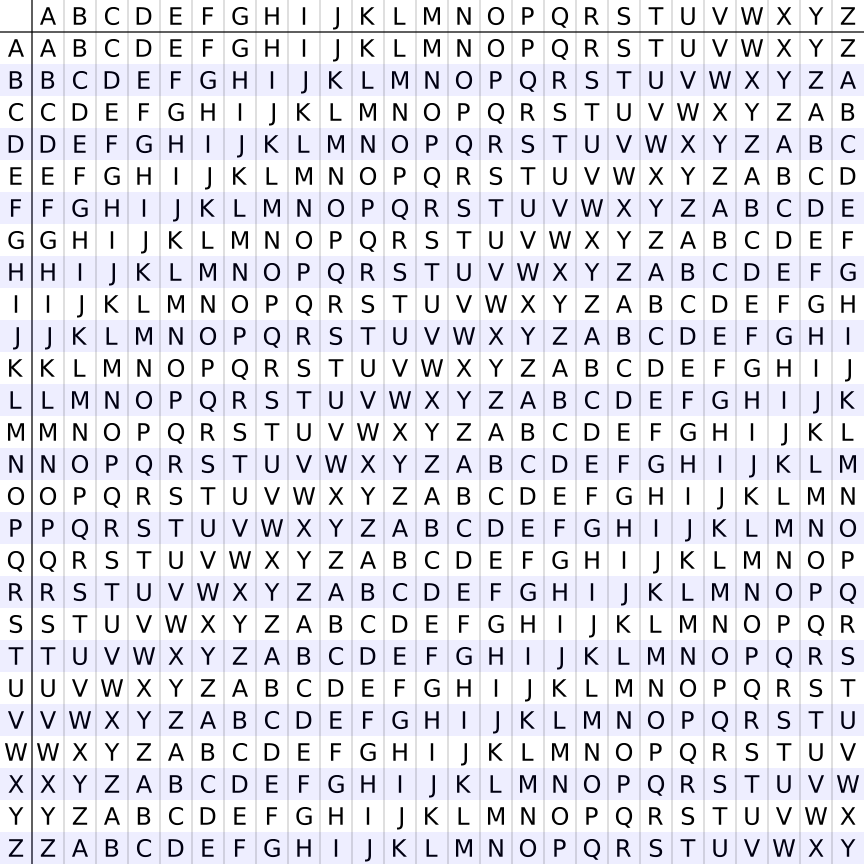
\includegraphics[scale=0.4]{tabula_recta}
\centering
\caption{A \textit{tabula recta}, which creates 26 different Caesar ciphers.}
\centering
\end{figure}
\ \\
The \textit{tabula recta} is often referred to when discussing pre-computer ciphers, such as the Vigenère cipher and Blaise de Vigenère's less well-known autokey cipher. Moreover, it can be proved that all polyalphabetic ciphers based on Caesar ciphers can be described in terms of the \textit{tabula recta}.\\\\
The encryption (and also the decryption) works like this: each letter of the message is switched with the letter directly below, using the first shifted alphabet. The next letter is switched by using the second shifted alphabet, and so on until the message is completely encrypted.\\\\
The resulting ciphertext looks like a random string; however, the letter frequencies are just shifted. For instance, if \textsf{e} is the most frequent letter in the cleartext and the shift is 3, then \textsf{h} will be the most frequent letter in the ciphertext.\\\\
Especially if the attacker is aware that this method is being used, it becomes extraordinarily easy to break. In fact, the cipher is considered vulnerable because it doesn't have a key.

\section{Vigenère cipher}
The \textbf{Vigenère cipher} is the best-known example of a polyalphabetic substitution cipher, which encrypts text by using a series of interwoven Caesar ciphers based on the letters of a keyword\supercite{vigenere1}.\\\\
The power of this cipher is that it's fairly easy to understand and implement, but it was considered unbreakable for three centuries\supercite{vigenere2}, earning this way the nickname \textit{le chiffre indéchiffrable} (French for `the indecipherable cipher').\\\\
It was originally described by Giovan Battista Bellaso in 1553, but the scheme was later misattributed to Blaise de Vigenère in the 19th century and so acquired its present name. The first man to describe a general method of breaking this cipher was Friedrick Kasiski in 1863.\\\\

\begin{figure}[H]
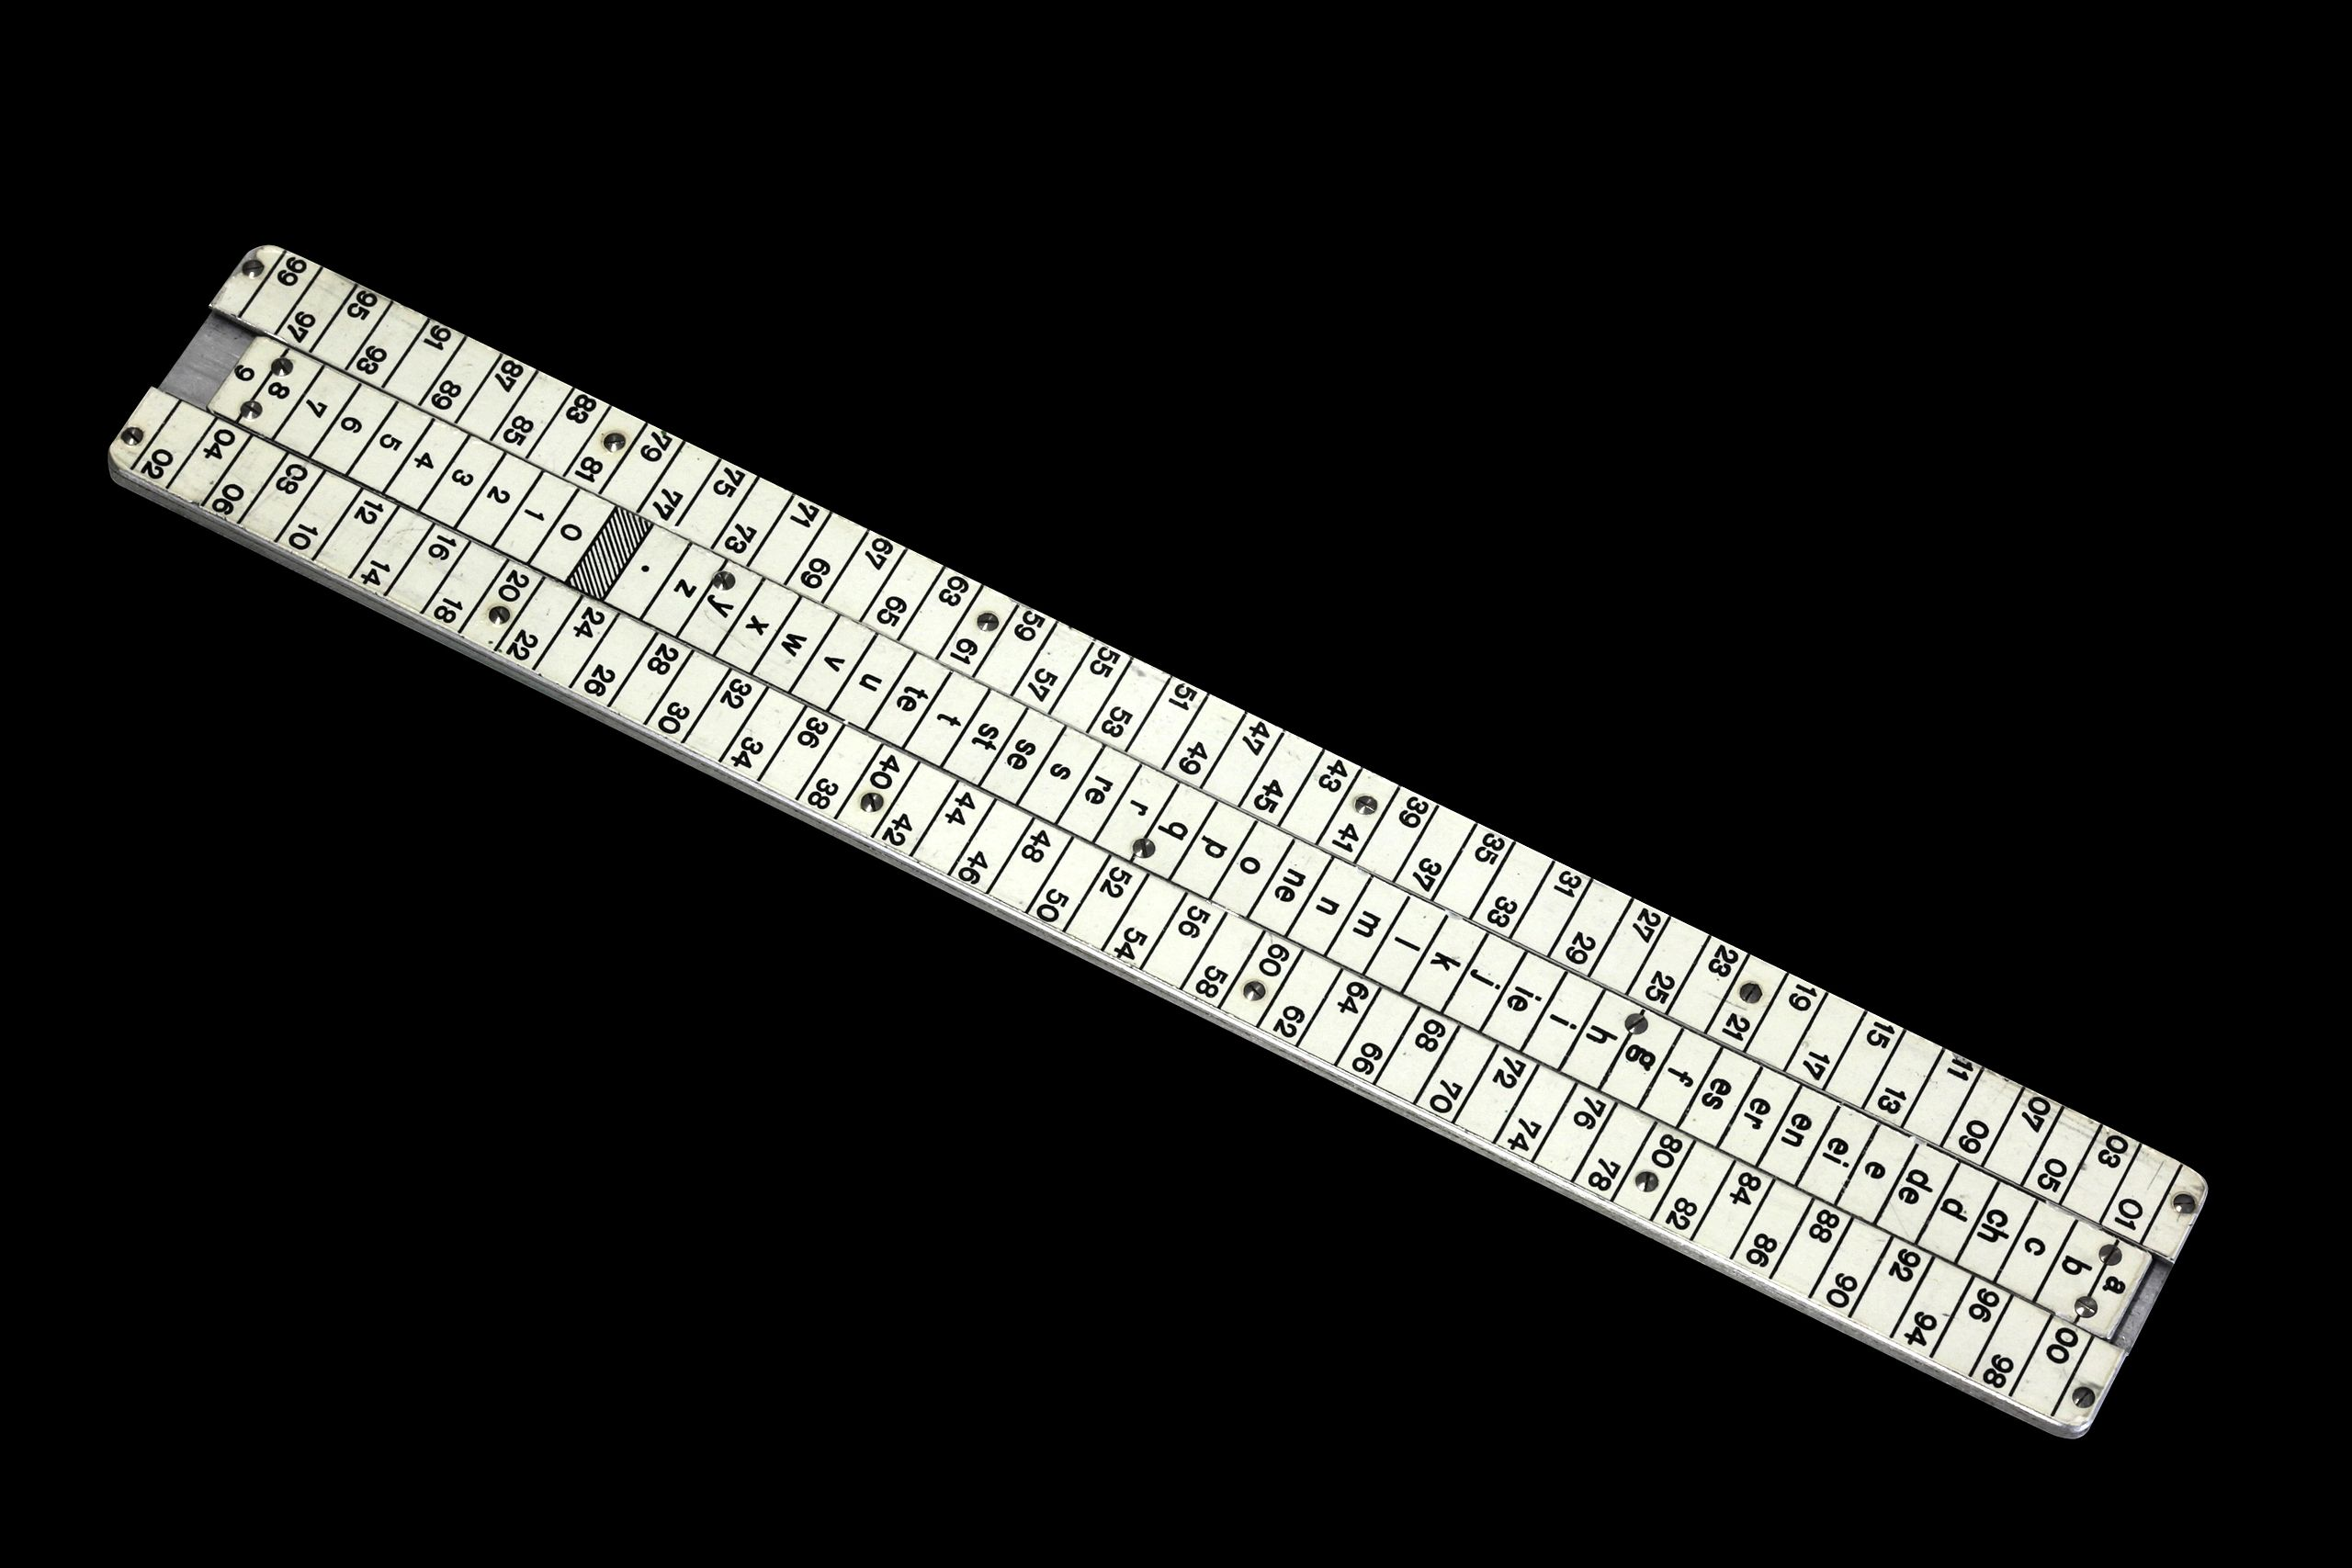
\includegraphics[scale=0.13]{slide_rule}
\captionsetup{justification=centering, margin=2cm}
\centering
\caption{Cryptographic slide rule used as a calculation aid by the Swiss Army between 1914 and 1940.}
\centering
\end{figure}

\ \\
The cipher makes large use of the \textit{tabula recta}: at different points in the encryption process, the cipher uses a different alphabet from one of the rows. A repeating keyword determines the alphabet used at each point\supercite{vigenere3}.\\\\
For example, suppose that the message to be encrypted is: \\\\
\colorbox{gray!12}{\small{\texttt{ATTACKATDAWN}}}\\\\
The sender chooses a keyword and repeats it until it matches the length of the plaintext; for instance, the keyword \textsf{LEMON}:\\\\
\colorbox{gray!12}{\small{\texttt{LEMONLEMONLE}}}\\\\
Each row starts with a key letter. Although there are 26 key rows shown, a code will use only as many different alphabets as there are unique letters in the keyword, here just 5: \textsf{L}, \textsf{E}, \textsf{M}, \textsf{O}, \textsf{N}. For successive letters of the message, successive letters of the keyword will be taken and each message letter enciphered by using its corresponding key row. The next letter of the key is chosen. and that row is gone along to find the column heading that matches the message character. The letter that lies at the intersection of key row and message column is the enciphered letter.\\\\
For example, the first letter of the plaintext, \textsf{A}, is paired with \textsf{L}, the first letter of the key. Therefore, row \textsf{L} and column \textsf{A} of the \textit{tabula recta} are used, i.e.\ \textsf{L}. Similarly, the intersection between row \textsf{E} and column \textsf{T} gives \textsf{X} as the enciphered letter. The rest of the message is encrypted likewise:\\\\
Plaintext: \par\colorbox{gray!12}{\small{\texttt{ATTACKATDAWN}}}\\\\
Key: \par\colorbox{gray!12}{\small{\texttt{LEMONLEMONLE}}}\\\\
Ciphertext: \par\colorbox{gray!12}{\small{\texttt{LXFOPVEFRNHR}}}\\\\

Decryption is performed in a similar fashion: once discovered the row in the table corresponding to the key letter, it's a matter of finding the position of the ciphertext letter in that particular row and then using the column's label as the plaintext. For example, in row \textsf{L} (from \textsf{LEMON}), the ciphertext \textsf{L} appears in column \textsf{A}. Thus \textsf{A} is the first plaintext letter.

\subsection{Algebraic description}
The Vigenère cipher can be marvelously described algebraically. Once transformed all the letters into their correspondent numbers, $A \rightarrow 0, B \rightarrow 1, ... , Z \rightarrow 25$, the encryption $E$ and the decryption $D$ using the key $K$ can be written as:

\begin{equation}
C_i=E_k{(M_i)}=(M_i + K_i) \ mod \ 26
\end{equation}
\begin{equation}
M_i=D_k{(C_i)}=(C_i - K_i) \ mod \ 26
\end{equation}
\ \\
in which $M = M_1 ... M_n$ is the message, $C = C_1 ... C_n$ is the ciphertext and $K = K_1 ... K_n$ is the key obtained by repeating the keyword.\\\\
The following is a \textsf{Python 2.7.x} implementation of a Vigenère cipher (note that the example used in the \texttt{main} function is the same as above, as well as the results of the \texttt{print} calls).\\\\
\pythonic{code/vigenere_cipher.py}
\ \\
\subsection{Gronsfeld cipher}
The \textbf{Gronsfeld cipher} is essentially identical to the Vigenère except for the fact that only 10 alphabets are used (i.e., only 10 rows of the \textit{tabula recta}). In doing so, a numerical keyword is often used (e.g. \textsf{40295} instead of \textsf{LEMON}), so that the number of rows of the table strictly matches the number of different values a digit can have.

\subsection{Beaufort cipher}
The \textbf{Beaufort cipher} is another variant of the Vigenère cipher, with a different enciphering mechanism and tableau (\textit{tabula recta}). It became popular thanks to its application in a rotor-based cipher machine, the Hagelin M-209.\\\\
The tableau on which this encryption scheme is based is practically the same as the one used in the Vigenère, but in reverse order starting with the letter \textsf{Z} in the first row, where the first row and the last column serve the same purpose.\\\\

\begin{figure}[H]
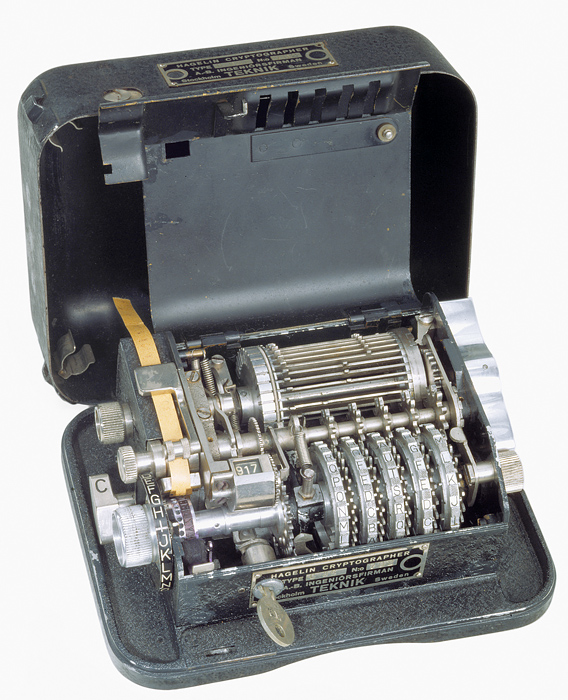
\includegraphics[scale=0.27]{m-209}
\captionsetup{justification=centering, margin=0.6cm}
\centering
\caption{The M-209, a mechanical cipher used by the US military in World War Two and the Korean War, designed by Swedish cryptographer Boris Hagelin.}
\centering
\end{figure}

\section{Autokey cipher}
With the definition of \textbf{autokey cipher}, we name all the ciphers that include the plaintext into the key used to encrypt. The key can be generated from the message in fancy ways: one of the most used alternative is that of adding a short \textit{primer key} to the front of the message.\\\\
This cipher was invented in 1586 by Blaise de Vigenère, although his initial version used an agreed-upon letter of the alphabet as a primer, which made the key along with the rest the message.\\\\
The encryption and decryption mechanisms, at least in more popular autokeys, follow the scheme of the Vigenère cipher, as well as the usage of a \textit{tabula recta}.\\\\
For example, if we have to transmit the message \colorbox{gray!12}{\small{\texttt{ATTACKATDAWN}}} and our \textit{primer key} is \textsf{QUEENLY}, then the key is \colorbox{gray!12}{\small{\texttt{QUEENLYATTACKATDAWN}}}; the key is consequently used as in the Vigenère cipher to encode the plaintext.

\subsection{Security for autokey ciphers}
Autokey ciphers are vastily considered more secure than ciphers that use fixed keys; this is due to the fact that the key doesn't repeat itself within a single message. Powerful cryptanalysis examinations, like the Kasiski's one or the index of coincidence, don't work on the ciphertext\supercite{autokey}, although they are very effective for similar ciphers that use a single repeated key.\\\\
Autokey ciphers, however, have a major weakness in the inclusion of the plaintext into the key. This means that the key is likely to contain common words at various points. The cipher can be attacked by using words, bigrams, trigrams etc. and by moving them until potentially-readable text comes out.\\
\section{Running key cipher}
A \textbf{running key cipher} is a substitution cipher in which a text (e.g., from a book) or passage is used to provide a long keystream. In most cases, the book is agreed upon ahead of time, while the passage is chosen randomly for each message. The encryption scheme is the same as the Vigenère cipher, thus the tableau used is the \textit{tabula recta}.\\\\
For example, if we have to encrypt \colorbox{gray!12}{\small{\texttt{Where shall we meet and at what time}}} and we choose “The Code Book by Simon Singh, starting at page 45, line 1” as our passage, our keystream would be \textsf{for centuries, the simple monoalphabetic substitution cipher had been sufficient to ensure secrecy}. We get the ciphertext:\\\\
\textbf{Ciphertext}: \colorbox{gray!12}{\small{\texttt{BVVTI FAUCT AWFLI LIZSL XIVNH XEFMB TTBLX}}}\\\

\subsection{Security for running key ciphers}
Unlike the Vigenère cipher, if the message is extended, the key is not repeated; in fact, if the running key is truly random, never reused, and secret, the result is a one-time pad, a method that provides perfect secrecy (i.e. reveals no information about the plaintext). However, if the running key is a block of text in a natural language, security actually becomes fairly poor, since that text will have non-random peculiarities which can be used to improve cryptanalysis. The low entropy per character makes the combining operation easy to be inverted.\\\\
To attack the cipher, a cryptanalyst runs guessed probable plaintexts along the ciphertext, subtracting them out from each possible solution. When the result is a chunk of something intelligible, there is a high chance that the guessed plaintext is correct for that position.\\\\
There are lots of different ways to improve the security of a running key cipher: the most obvious one is to use a secret mixed alphabet tableau instead of a classical \textit{tabula recta}. This does indeed complicate matters but it's not a complete solution. Another possibility is to use a key text that has higher entropy per character than typical English: for example, documents such as almanacs and trade reports often contain long lists of random-looking numbers.\\\\
Another problem is that the keyspace is surprisingly small. Suppose that there are 100 million key texts that might plausibly be used, and that on average each has 11'000 possible starting positions. To an opponent with a massive collection of possible key texts, this leaves possible a brute force search of the order of $2^{40}$, which by computer cryptography standards is a relatively easy target.

\chapter{Other classes of substitution ciphers}
\section{Homophonic ciphers}
\textbf{Homophonic substitution} was an early attempt to make monoalphabetic substitution ciphers harder to break. The basic idea behind homophonic substitution is to allocate \textbf{more than one letter or symbol} to the higher frequency letters\supercite{homophonic}. For example, we might use 6 different symbols to encrypt \textsf{e} and \textsf{t}, 2 symbols for \textsf{m} and only 1 symbol for \textsf{z}.\\\\
Since more than 26 characters will be required in the ciphertext alphabet, various solutions are employed to invent larger alphabets. The standard way to do this is to include the numbers in the ciphertext alphabet, but we could also use a mixture of uppercase, lowercase, and upside down letters. Some cryptographers even design artistic symbols to use.\\\\
The easiest way to break standard substitution ciphers is to look at the letter frequencies: the letter \textsf{E} is usually the most common letter in English, followed by \textsf{T}. If we allow the letter \textsf{E} to be replaced by any of 4 different characters, then we can no longer just take the most common letter in the ciphertext, since the letter count of \textsf{E} is spread over several characters. As we allow more and more possible alternatives for each letter, the resulting cipher becomes more and more secure.\\\\
For example, let's consider our cipher alphabet as follows:

\begin{figure}[H]
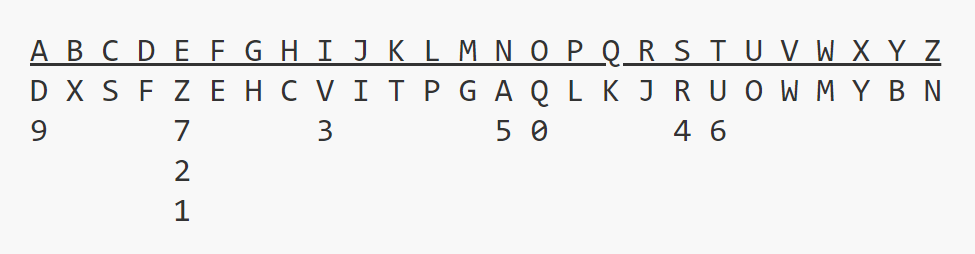
\includegraphics[scale=0.4]{homophonic_cipher}
\centering
\caption{}
\centering
\end{figure}

To encipher the message \textsf{DEFEND THE EAST WALL OF THE CASTLE}, we find the letter \textsf{D} in the top row. then replace it with the letter below it, \textsf{F}. The second letter, \textsf{E}, provides us with several choices: we could use any of \textsf{Z}, \textsf{7}, \textsf{2} or \textsf{1}. We choose one of these at random, say \textsf{7}. After continuing with this, we get the ciphertext:\\
\ \\
\textbf{Plaintext}: \par\colorbox{gray!12}{\small{\texttt{DEFEND THE EAST WALL OF THE CASTLE}}}\\\\
\textbf{Ciphertext}: \par\colorbox{gray!12}{\small{\texttt{F7EZ5F UC2 1DR6 M9PP 0E 6CZ SD4UP1}}}\\

The number of ciphertext letters assigned to each plaintext letter was chosen to flatten the frequency distribution as much as possible. Since \textsf{E} is normally the most common letter, it is allowed more possibilities so that the frequency peak from the letter \textsf{E} will not be present in the ciphertext.\\\\
Breaking homophonic substitution ciphers can be very difficult if the number of homophones is high. The usual method is some sort of hill climbing, an algorithm which uses the fitness of a deciphered text to improve the decryption itself. In addition to finding which letters map to which others, we also need to determine how many letters each plaintext letter can become.

\subsection{Book cipher}
A \textbf{book cipher} is a cipher in which the key is some aspect of a book or other piece of text. Traditionally book ciphers work by replacing word in the plaintext of a message with the location of words from the book being used; in this mode, book ciphers are more properly called \textit{codes}. This approach can have problems, since a word which appears in the plaintext but not in the book cannot be encoded\supercite{book_cipher}.\\\\

\begin{figure}[H]
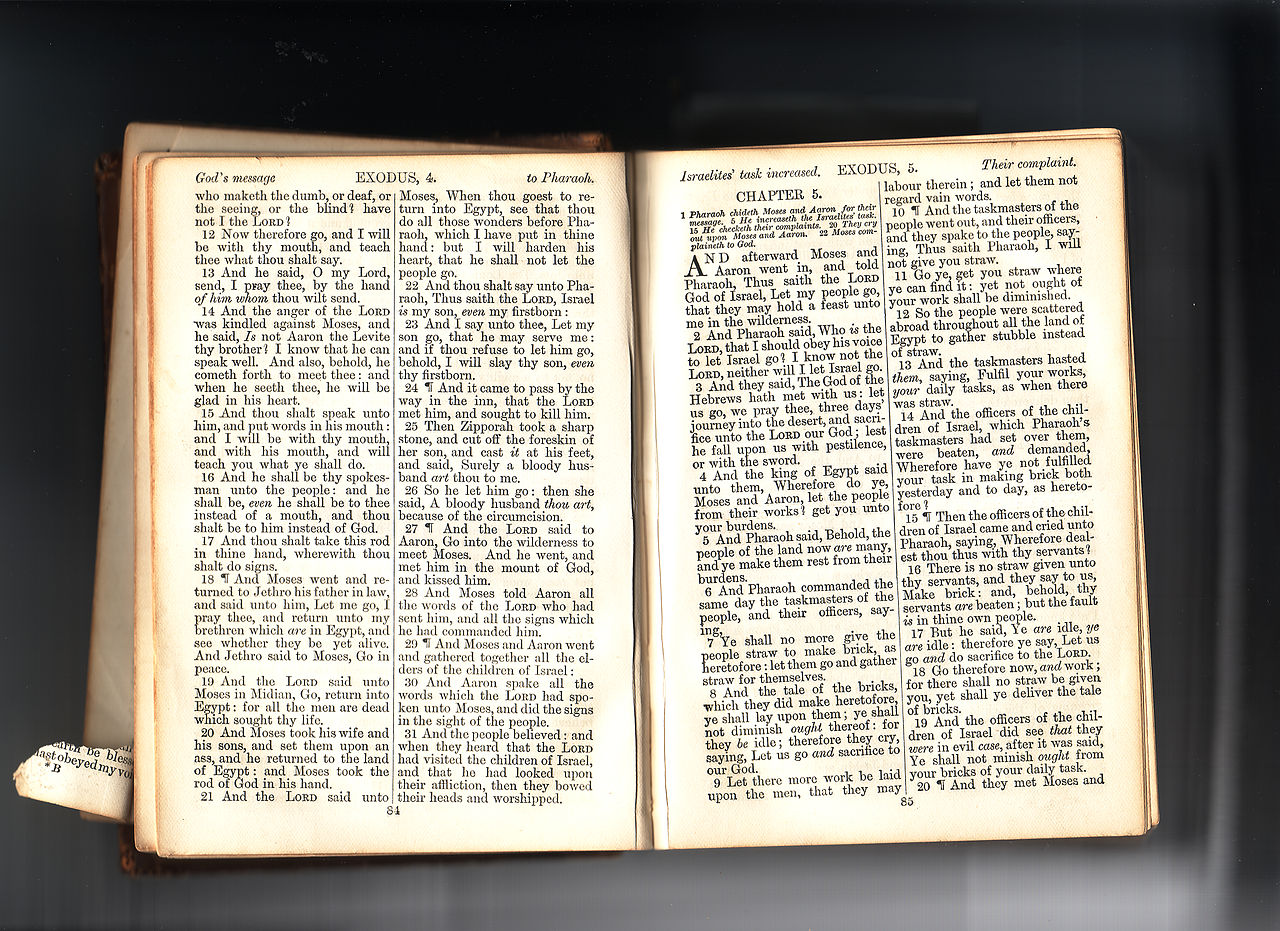
\includegraphics[scale=0.9]{king_james_bible}
\captionsetup{justification=centering, margin=2cm}
\centering
\caption{The King James Bible, a highly available publication suitable for the book cipher.}
\centering
\end{figure}
\ \\
A famous use of a book cipher is in the \textit{Beale ciphers}, a set of three ciphertexts, one of which allegedly states the location of a buried treasure estimated to worth over \$43 million. The second document, in fact, uses the United States Declaration of Independence as the key text.\\\\
An alternative approach is, for example, that of replacing the first letter of a word in the book with that word's position; in this case, the book is cipher is properly a homophonic substitution cipher. However, if used often, this technique has the side effect of creating a larger ciphertext and increases the time and effort required to decode the message.

\section{Polygraphic ciphers}
A \textbf{polygraphic substitution} is a cipher in which a uniform substitution is performed on blocks of letters. When the length of the block is specifically known, more precise terms are used: for instance, a cipher in which pairs of letters are substituted is called digraphic.\\\\
As a concept, polygraphic substitution contrasts with monoalphabetic substitution, in which individual letters are uniformly substituted, and polyalphabetic substitution, in which individual letters are substituted using multiple alphabets. In a polygraphic substitution cipher, plaintext letters are substituted in larger groups. The first advantage is that the frequency distribution is much flatter than that of individual letters (though not actually flat in real languages; e.g., \textsf{TH} is much more common that \textsf{EQ} in English. Second, the larger number of symbols requires correspondingly more ciphertext to productively analyze letter frequencies. In order to substitute pairs of letters, it would take a substitution alphabet composed of 676 symbols ($26^{2}$).

\subsection{Playfair cipher}
The \textbf{Playfair cipher} was the first cipher to encrypt pairs of letters in cryptologic history. Charles Wheatstone invented it in 1854 for secrecy in telegraphy, but it bears the name of Lord Playfair who promoted its use\supercite{playfair}. The Playfair cipher has been largely used for tactical purposes by British forces in the Second Boer War, in World War I and in World War II: this was because Playfair is reasonably fast to use and requires no special equipment - just a pencil and some paper.\\\\
The Playfair cipher uses a $5 \times 4$ table containing a key word or phrase. Memorization of the keyword and 4 simple rules was all that was required to create the table and use the cipher. To generate the key table, one would first fill in the spaces in the table with the letters of the keyword, dropping any duplicate letters, and then fill the remaining spaces with the rest of the letters of the alphabet in order (sometimes putting both I and J in the same space to reduce the alphabet to fit).\\\\
To encrypt a message, one would break the message into digrams, which will be substituted using the key table. To perform the substitution, we have to apply the following rules, in order, to each digram in the plaintext:

\begin{itemize}
	\item If both letters are the same (or only one letter is left in the plaintext), add an \textsf{X} after the first letter; encrypt the new pair and continue.
	\item If the letters appear on the same row of the table, replace them with the letters to their immediately right respectively, wrapping around to the left side of the row if a letter in the original pair was on the right side of the row.
	\item If the letters appear on the same column of the table, replace them with the letters immediately below respectively, wrapping around to the top side of the column if a letter in the original pair was on the bottom side of the column.
	\item If the letters are not on the same row or column, replace with the letters on the same row respectively but at the other pair of corners of the rectangle defined by the original pair. The order is important - the first letter of the encrypted pair is the one that lies on the same row as the first letter of the plaintext.
\end{itemize}

To decrypt, we have to use the inverse of the last 3 rules, and the first as-is (dropping any extra \textsf{X}s that do not make sense in the final message when finished).\\\\

\subsubsection{Example}
We'll use \textsf{playfair example} as the key of our cipher; the table becomes (omitted letters in red):\\\\
\begin{figure}[H]
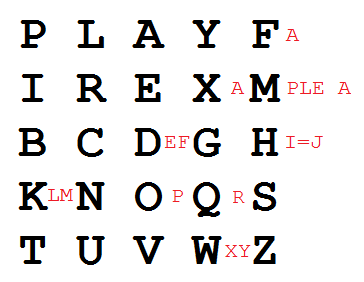
\includegraphics[scale=0.8]{playfair_example}
\centering
\caption{}
\centering
\end{figure}
\ \\
The message we have to encrypt is \textsf{Hide the gold in the tree stump}. After dividing the message in digrams, we analyze three of them which represent different scenarios.\\\\
\begin{figure}[H]
\minipage{0.28\textwidth}
  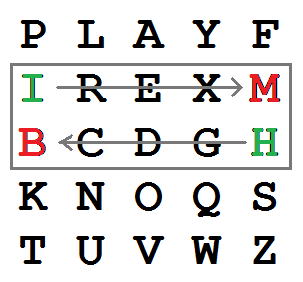
\includegraphics[width=\linewidth]{playfair_1}
  \caption{The digram HI, which is the first digram of the plaintext), is replaced by BM; this is the rectangle scenario (last rule).}
\endminipage\hfill
\minipage{0.28\textwidth}
  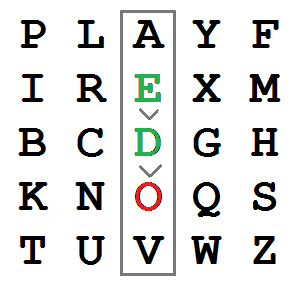
\includegraphics[width=\linewidth]{playfair_2}
  \caption{The digram DE, which is the second digram of the plaintext, is replaced by OD; this is the same-column scenario.}
\endminipage\hfill
\minipage{0.28\textwidth}%
  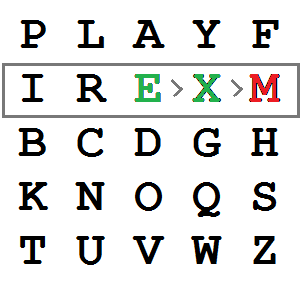
\includegraphics[width=\linewidth]{playfair_10}
  \caption{The digram EX, which is the tenth digram of the plaintext after applying the first rule, is replaced by XM; this is the same-row scenario.}
\endminipage
\end{figure}
\ \\
\textbf{Ciphertext}: \colorbox{gray!12}{\small{\texttt{BM OD ZB XD NA BE KU DM UI XM MO UV IF}}}\\\\

\subsubsection{Cryptanalysis}
If there's enough text available, the Playfair cipher can be easily cracked. When only the ciphertext is known, brute force cryptanalysis of the cipher involves searching through the key space for matches between the frequency of occurrence of digrams and the known frequency of occurrence of digrams in the assumed language of the original message.\\\\
A different approach to tackling a Playfair cipher is the shotgun hill climbing method. This starts with a random square of letters; then minor cchanges are introduced (e.g. switching letters or rows) to see if the candidate plaintext is more like standard plaintext than before the change. If the new square is deemed to be an improvement, then it is adopted and further mutated to find an even better candidate. Eventually, the plaintext or something very close is found to achieve a maximal score by whatever grading method is chosen. This is obviously beyond the range of typical human patience, but computers can adopt this algorithm to crack Playfair ciphers with a relatively small amount of text.\\\\

\subsection{Hill cipher}
The \textbf{Hill cipher} was invented by Lester S. Hill in 1929, and like other polygraphic ciphers, it can work on digraphs, trigraphs or theoretically any sized blocks. This cipher uses linear algebra, and has a significantly more mathematical nature than some of the others\supercite{hill}. However, it is this nature that allows it to act easily on larger blocks of letters.\\\\
To encrypt a message using the Hill cipher we must first turn our keyword into a key matrix (a $2 \times 2$ matrix for working with digraphs, a $3 \times 3$ matrix for working with trigraphs, etc). We also turn the plaintext into digraphs (or trigraphs) and each of these into a column vector. We then perform matrix multiplication modulo the length of the alphabet on each vector. These vectors are then converted back into letters to produce the ciphertext.\\\\
We shall encrypt the plaintext message \colorbox{gray!12}{\small{\texttt{short example}}} using the keyword \textsf{hill}: the first step is to turn the keyword into a matrix. If the keyword was longer than the 4 letters needed, we would only take the first 4 letters, and if it was shorter, we would fill it up with the alphabet in order. We then convert this into a key matrix using the standard convention of positions of letters in the alphabet.\\\\
\begin{equation}
\begin{pmatrix}
	H & I \\
	L & L
\end{pmatrix}
\rightarrow
\begin{pmatrix}
	7 & 8\\
	11 & 11
\end{pmatrix}
\end{equation}
\ \\\\
We now split the plaintext into digraphs, write these as column vectors, and apply the same conversion method used to transform the keyword into the key matrix.\\\\
\begin{equation}
\begin{pmatrix}s\\h\end{pmatrix}
\begin{pmatrix}o\\r\end{pmatrix}
\begin{pmatrix}t\\e\end{pmatrix}
\begin{pmatrix}x\\a\end{pmatrix}
\begin{pmatrix}m\\p\end{pmatrix}
\begin{pmatrix}l\\e\end{pmatrix}
\rightarrow
\begin{pmatrix}18\\7\end{pmatrix}
\begin{pmatrix}14\\17\end{pmatrix}
\begin{pmatrix}19\\4\end{pmatrix}
\begin{pmatrix}23\\0\end{pmatrix}
\begin{pmatrix}12\\15\end{pmatrix}
\begin{pmatrix}11\\4\end{pmatrix}
\end{equation}
\ \\\\
Now we must perform some matrix multiplication. We multiply the key matrix by each column vector in turn, then we apply the modulo 26 and then convert the numbers back to letters. For example, the first digram of the plaintext, \textsf{sh}, becomes:\\\\
\begin{equation}
\begin{pmatrix}H&I\\L&L\end{pmatrix}\begin{pmatrix}s\\h\end{pmatrix}=
\begin{pmatrix}7&8\\11&11\end{pmatrix}\begin{pmatrix}18\\7\end{pmatrix}=
\begin{pmatrix}182\\275\end{pmatrix}=
\begin{pmatrix}0\\15\end{pmatrix} \ mod \ 26=
\begin{pmatrix}A\\P\end{pmatrix}
\end{equation}
\ \\\\
The final ciphertext is: \colorbox{gray!12}{\small{\texttt{APADJ TFTWLFJ}}}\\\\
To decrypt a ciphertext encoded using the Hill cipher, we must find the inverse key matrix (not an easy task): once we have the inverse matrix, the process is the same as encrypting (i.e. we multiply the inverse key matrix by the column vectors that the ciphertext is split into, take the results modulo the length of the alphabet, and finally convert the numbers back to letters.\\\\
In general, to find the inverse of the key matrix, we perform the calculation below, where $K$ is the key matrix, $d$ is its determinant, and $adj{(K)}$ is the adjugate matrix of $K$ (everything taken modulo 26).\\\\
\begin{equation}
K^{-1} = d^{-1} \times adj{(K)}
\end{equation}
\ \\
\subsubsection{Step 1 - Find the multiplicative inverse of the determinant}
We first calculate the determinant modulo 26, which is pretty straightforward for a $2 \times 2$ matrix:\\\\
\begin{equation}
\begin{vmatrix}7&8\\11&11\end{vmatrix} = 7 \times 11 - 8 \times 11 = -11 = 15 \ mod \ 26
\end{equation}
\ \\\\
We now have to find the multiplicative inverse of the determinant working modulo 26, which is the number $d^{-1}$ between 1 and 25 that gives a result of 1 when we multiply it by $d$:\\\\
\begin{equation}
d d^{-1} = 1 \ mod \ 26
\end{equation}
\ \\\\
There are several algorithms to efficiently calculate this number, but it is often easiest to use trial and error to find the inverse. In this case, we obtain that the number we're looking for is 7, since $15 \times 7 = 105 = 1 \ mod \ 26$

\subsubsection{Step 2 - Find the adjugate matrix}
The adjucate matrix is a matrix of the same size of the original; we won't give additional details on this, but for a $2 \times 2$ matrix it is fairly simple as it is just moving the elements to different positions and changing a couple of signs. That is, we swap the top left and bottom right numbers in the key matrix, and change the sign of the top right and bottom left number. Algebraically this is given below:\\\\
\begin{equation}
adj\begin{pmatrix}a&b\\c&d\end{pmatrix} = \begin{pmatrix}d&-b\\-c&a\end{pmatrix}
\end{equation}
\ \\\\
Again, once we have these values we will need to take each of them modulo 26 (in particular, we need to add 26 to the negative values to get a number in the range from 0 to 25). For our example we get the matrix below:\\\\
\begin{equation}
adj \begin{pmatrix} 7 & 8 \\ 11 & 11 \end{pmatrix} = 
\begin{pmatrix} 11 & -8 \\ -11 & 7 \end{pmatrix} = 
\begin{pmatrix} 11 & 18 \\ 15 & 7 \end{pmatrix} \ mod \ 26
\end{equation}
\ \\
\subsubsection{Step 3 - Multiply the multiplicative inverse of d by the adjugate matrix}
To get the inverse key matrix, we now multiply the inverse determinant (that was 7 in our case) from step 1 by each of the elements of the adjugate matrix from step 2. Then we take each of these values modulo 26:\\\\
\begin{equation}
K^{-1} = 7 \times \begin{pmatrix} 11 & 18 \\ 15 & 7 \end{pmatrix} =
\begin{pmatrix} 77 & 126 \\ 165 & 49 \end{pmatrix} = \begin{pmatrix} 25 & 22 \\ 1 & 23 \end{pmatrix} \ mod \ 26
\end{equation}
\ \\\\
Now that we have the inverse key matrix, we can easily convert the ciphertext back to plaintext using the same method adopted in the encryption process. For example, for the first digram \textsf{AP}, corresponding to $(0, 15)$ we have:\\\\
\begin{equation}
\begin{pmatrix} 25 & 22 \\ 1 & 23 \end{pmatrix} \begin{pmatrix} 0 \\ 15 \end{pmatrix} = 
\begin{pmatrix} 330 \\ 345 \end{pmatrix} = \begin{pmatrix} 18 \\ 7 \end{pmatrix} \ mod \ 26 \rightarrow \begin{pmatrix} s \\ h \end{pmatrix}
\end{equation}
\ \\\\
The key matrix must have a non-zero determinant which is coprime to the length of the alphabet. In fact, if $d$ is 0, then we cannot compute an inverse key matrix, and if $GCD(d, m)$ is not 1 ($m$ is the length of the alphabet), the multiplicative inverse of the determinant wouldn't exist.\\\\
The security of the Hill cipher increases as the key matrix size increases: however, the complexity of operating the cipher increases as well. Hill invented a machine that would mechanically implement a $6 \times 6$ version of the cipher, which was very secure. Unfortunately, the machine was unable to change the key setting, leaving it with limited use in the real world.\\\\
Cryptanalysis of an intercept encrypted using the Hill Cipher is certainly possible, especially for small key sizes. For the $2 \times 2$ version, looking for repeated digraphs would be the first step, and matching the most common ciphertext digraphs to the most common digraphs in English would allow the interceptor to put together a possible key matrix acting on those four letters.

\chapter{Breaking substitution ciphers: standard techniques}
When breaking an unknown cipher, one first needs to figure out what kind of cipher one it is. Generally, a good starting point would be to start with the most common and well-known classical ciphers, drop those that obviously don't fit, and try the remaining ones to see if any of theme might work.\\\\
An obvious first step is to look at the ciphertext alphabet: does the ciphertext consist of letters (and if so, in what alphabet), numbers, abstract symbols or some combination of those? If it's letters, does it include spaces, punctuation or case distinctions - and, if it does, do they seem to be scrambled in some way, or are they maybe just left as they are in the plaintext?\\\\
Compiling a letter (or symbol) frequency table of the ciphertext, and comparing it to the corresponding table of plain English text, can often yield important information about the general type of cipher one is dealing with:

\begin{itemize}
	\item If the ciphertext is written in letters, and their frequencies more or less match those of plain English text, we're probably dealing with a transposition cipher, by which the positions held by units of plaintext are shifted according to a regular system, so that the ciphertext constitutes a permutation of the plaintext. Moreover, if the most frequent letters don't quite match. but still look plausible for natural text - mostly vowels and a few simple consonants - it might be a transposition of text in some other language.
	\item If the rank-frequency distribution looks similar to that for plain English, but the letters are scrambled, the cipher is very likely to be a monoalphabetic substitution one, possibly combined with transposition.
	\item If the frequency distribution is closer to uniform than one would expect for natural language, we're probably looking at a polyalphabetic substitution cipher. With experience and enough ciphertext, one may even be able to guess at the most likely cipher just based on the frequency distribution.
\end{itemize}
\ \\
Knowing whether the cipher has a key or not, and what form the key takes (word, number, sequence of numbers, etc.) can also help reduce the range of possibilities. For example, say that the ciphertext is uppercase letters without spaces or punctuation, and that we know it has a key which is a word or a short phrase. That narrows down the likely choices quite a bit:

\begin{itemize}
	\item If it's a \textit{transposition cipher}, the obvious thing to try would be columnar transposition and its variants like double transposition.
	\item If it's a \textit{monoalphabetic substitution cipher} and has a keyword, the keyword cipher (described at the beginning of the first chapter) is the natural choice.
	\item If it's a \textit{polyalphabetic substitution}, there are more choices. The first cipher to try out would be Vigenère and autokey; if those don't work out, Beaufort may be worth trying too.
\end{itemize}
\ \\
When one already knows what the key is supposed to be, testing each cipher should be pretty straightforward: one would just try to decrypt the message with the key and see if the output of that operation makes sense.\\\\
Note that, in some seldom cases, effort can be shared between ciphers. For example, the Vigenère and autokey ciphers are identical for the beginning of the message; they only start to behave differently when the end of the keyword is reached. It may also be a good idea to try simple variants of these ciphers, such as switching the encryption and decryption rules around; some of them work equally well in both directions, and may have been used so.

\section{Frequency analysis}
The methodology behind \textbf{frequency analysis} relies on the fact that in any language, each letter has its own \textit{personality}. The most obvious trait that letters have is the frequency with which they appear in a language. Clearly in English the letter \textsf{Z} appears far less frequently than, say, \textsf{A}. In times gone by, if we wanted to find out the frequencies of letters within a language, we had to find a large piece of text and count each frequency. Now, however, we have computers that can do the hard work for us. But in fact, we don't even need to do this step, as for most languages there are databases of the letter frequencies, which have been calculated by looking at millions of texts, and are thus very highly accurate\supercite{digram_frequencies}.\\\\
From these databases we find that \textsf{E} is the most common letter in English, appearing about 12\% of the time (that is just over one in ten letters is an \textsf{E}). The next common letter is \textsf{T} at 9\%. The full frequency list is given by this graph:\\\\

\begin{figure}[H]
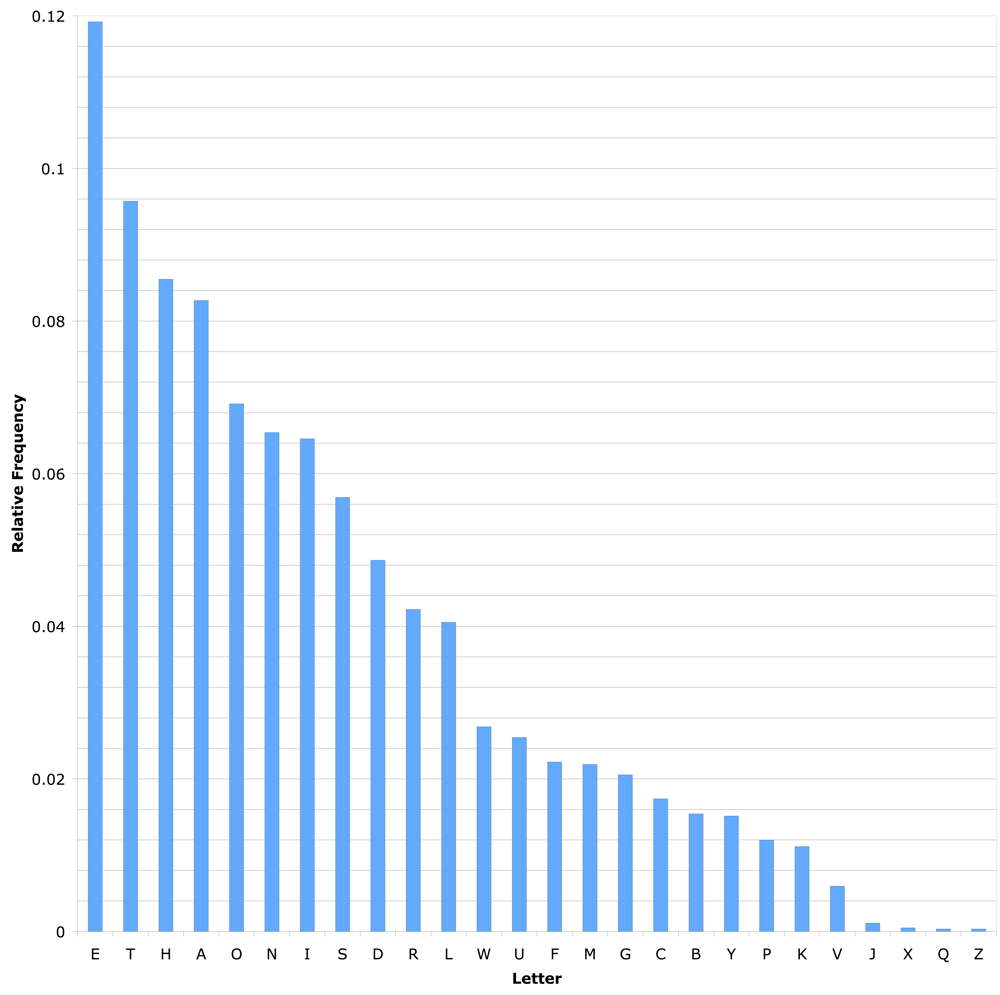
\includegraphics[scale=0.35]{letter_frequency}
\centering
\caption{Relative frequency for each letter of the English alphabet.}
\centering
\end{figure}
\ \\
We can use this information to help us break a code given by a monoalphabetic substitution cipher. This works because, if \textsf{e} has been encrypted to \textsf{X}, then every \textsf{X} was an \textsf{e}. Hence, the most common letter in the ciphertext should be \textsf{X}.\\\\
If we were to just put all the letters in order, and replace them as in the frequencies, it would likely produce jibberish, especially if the ciphertext is short. The codebreaker has to use other `personality traits' of the letters to decrypt the message. This may include looking at common digraphs: there aren't many 2 letter words, and there are only a few letters which appear as doubles (\textsf{SS}, \textsf{EE}, \textsf{TT}, \textsf{LL}, \textsf{OO} and \textsf{FF} being the most common). Other common words also start to appear as we make more and more substitutions: for example, \textsf{tKe} might appear frequently after making substitutions for \textsf{t} and \textsf{e}. This is very likely to be \textsf{the}, the most common trigram in English.\\\\
The process of frequency analysis uses various subtle properties of the language, and for this reason, it is nearly impossible to have a computer do all the work. Inevitably, an element of human input is necessary in this process to make educated decisions about which letters to substitute.\\

\subsection{Worked example}
In this example we shall use frequency analysis to break the code used to encrypt the intercept given below, given that it has been encrypted with a monoalphabetic substitution cipher.\\

\begin{displayquote}\texttt{\small{GFSWM YOGLG DVSMF SFNKY HOSUE SLLMR SPCWS BFGWP OLDMF RQMRS PLOGC PFUMU PCCSK SFOHD MPFOS XOGCO ISLME SDMFR QMRSD GFRSF GQRIO GCPDD GFSLI SSOGK LGMFU OISFW SNGQF OOISG NNQKK SFNSL GCSMN IDSOO SKWSN MDDOI SEGLO CKSJQ SFODY GNNQK KPFRD SOOSK OISCP KLOOI SFSXO EGLOG NNQKK PFRDS OOSKO ISLSN GFUOI SCGDD GWPFR EGLOG NNQKK PFRDS OOSKO ISOIP KUMFU LGGFQ FOPDW SMNNG QFOCG KMDDO ISUPC CSKSF ODSOO SKLPF OISHD MPFOS XOLME HDSOI SFWSD GGBMO OISNP HISKO SXOWS WMFOO GLGDV SMFUW SMDLG NDMLL PCYPO LLYEA GDLWS CPFUO ISEGL OGNNQ KKPFR LYEAG DMFUN IMFRS POOGO ISCGK EGCOI SCPKL ODSOO SKGCO ISHDM PFOSX OLMEH DSOIS FSXOE GLONG EEGFL YEAGD PLNIM FRSUO GOISC GKEGC OISLS NGFUD SOOSK MFUOI SCGDD GWPFR EGLON GEEGF LYEAG DPLNI MFRSU OGOIS CGKEG COISO IPKUD SOOSK MFULG GFQFO PDWSM NNGQF OCGKM DDLYE AGDLG COISN KYHOG RKMEW SWMFO OGLGD VXXXX
}}
\end{displayquote}
\ \\
The first step is to find the frequency of all the letters appearing in the intercept, and compare it to the frequency of standard English.\\
\begin{figure}[H]
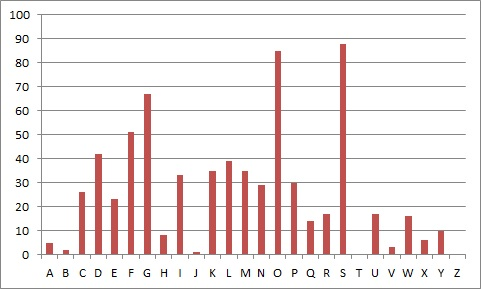
\includegraphics[scale=0.7]{frequency_analysis_example}
\centering
\caption{Letter frequencies in the ciphertext.}
\centering
\end{figure}
\ \\
Now that we have all the frequencies of ciphertext letters, we can start to make some substitutions. We see that the most common ciphertext letter is \textsf{S}, closely followed by \textsf{O}. From the chart above, we can guess that these two letters represent \textsf{e} and \textsf{t} respectively.\\\\
After replacing these letters (intermediate versions of the intercept are not shown due to its length), we notice that the word \textsf{tIe} is appearing frequently in the passage. In English, the most common 3 letter word is \textsf{the} and this fits what we have already done, which suggests that \textsf{I} should be decrypted to \textsf{h}.\\\\
Also, by looking at the frequencies again, we see the next most common letter is \textsf{G}, which is probably one of \textsf{a}, \textsf{i} or \textsf{o}. We see that the third word is \textsf{tG}, and the only one of these options that makes sense is \textsf{to}, so we guess \textsf{G} replaces \textsf{o}.\\\\
The first work is now \textsf{oFe}, which when considered with the appearance of \textsf{theF}, leads us to the conclusion that \textsf{F} is \textsf{n}; this also fits in with the frequencies of both letters in the tables.\\\\
After repeating these passages a few times, we can easily decrypt the whole intercept by looking at partially-solved words (\textsf{Lheet} instead of \textsf{sheet}, \textsf{enoQRh} instead of \textsf{enough}, etc). The plaintext, once solved, is an extract from `A manuscript on deciphering cryptographic messages` from around 850AD, which is the earliest known description of the process of frequency analysis:\\

\begin{displayquote}\textsf{{\small
One way to solve an encrypted message, if we know its language, is to find a different plaintext of the same language long enough to fill one sheet or so, and then we count the occurrences of each letter. We call the most frequently occurring letter the 'first', the next most occurring letter the 'second' the following most occurring letter the 'third', and so on, until we account for all the different letters in the plaintext sample. Then we look at the cipher text we want to solve and we also classify its symbols. We find the most occurring symbol and change it to the form of the 'first' letter of the plaintext sample, the next most common symbol is changed to the form of the 'second' letter, and the following most common symbol is changed to the form of the 'third' letter, and so on, until we account for all symbols of the cryptogram we want to solve.
}}
\end{displayquote}
\ \\
\section{Kasiski examination}
\textbf{Kasiski examination} is a method of attacking polyalphabetic substitution ciphers, named after Friedrich Kasiski who first published it in 1863, although it seems to have been independently discovered by Charles Babbage as early as 1846.\\\\
The strength of ciphers like Vigenère one (and derivatives) is that they're not susceptibe to frequency analysis, due to the fact that the cipher rotates through different shifts, so the same plaintext letter will not always be encrypted to the same ciphertext letter\supercite{kasiski}.\\\\
Nonetheless, there is one main weakness to the security of this kind of ciphers, and that's the fact that the key is repeated. If we use the keyword \textsf{key}, then the keystream will be a repetition of it; this means that we have 3 interwoven Caesar ciphers, which can be individually broken using frequency analysis. The hard part is thus working out the length of the keyword.\\\\
The solution that Kasiski came up with was ingenious. As an example, consider what we get when we encode the plaintext \colorbox{gray!12}{\small{\texttt{maths is short for mathematics}}} using the keyword \textsf{key}. When we use the Vigenère cipher, we can see that the ciphertext contains a repetition corresponding to the two times we see "math" in the plaintext.\\\\
As a cryptanalyst this gives us some useful information. Since the repeating key are 15 letters apart, we know that the length of the key must be a divisor of 15. That is, the keyword must be of the lengths 1, 3, 5, 15. Although it's theoretically possible to have keywords of length 1 or 15, we can drop these cases and focus on instances of keywords of length 3 and 5.\\\\
However, we have to consider the fact that it's possible for a string to repeat in the ciphertext as a pure coincidence. To increase our chances to find the length of the key, we can try to find more than one repeating string in the ciphertext, and computes the intersection of the sets describing the likely distances for every given string.\\\\
Obviously, the longer the message the more repeated n-graphs there are likely to be, and the more confident we can be about the length of the keyword. Once discovered the length of the keyword, we can write out the ciphertext in that many columns. For instance, if the keyword is 6 letters long, we can write the ciphertext in 6 columns and do a bit of frequency analysis on each column\supercite{kasiski_method}.\\\\
\subsection{Worked example}
In this example we shall use Kasiski examination in order to break the code used to encrypt the text below, given that a Vigenère cipher has been used.

\begin{displayquote}{\small{\texttt{CVJTN AFENM CDMKB XFSTK LHGSO JWHOF UISFY FBEXE INFIM AYSSD YYIJN PWTOK FRHWV WTZFX HLUYU MSGVD URBWB IVXFA FMYFY XPIGB HWIFH HOJBE XAUNF IYLJW DKNHG AOVBH HGVIN AULZF OFUQC VFBYN FTYGM MSVGX CFZFO KQATU IFUFE RQTEW ZFOKM WOJYL NZBKS HOEBP NAYTF KNXLB VUAXC XUYYK YTFRH RCFUY CLUKT VGUFQ BESWY SSWLB YFEFZ VUWTR LLNGI ZGBMS ZKBTN TSLNN MDPMY MIUBV MTLOB JHHFW TJNAU FIZMB ZLIVH MBSUW LBYFE UYFUF ENBRV JVKOL LGTVU ZUAOJ NVUWT RLMBA TZMFS SOJQX LFPKN AULJC IOYVD RYLUJ MVMLV MUKBT NAMFP XXJPD YFIJF YUWSG VIUMB WSTUX MSSNY KYDJM CGASO UXBYS MCMEU NFJNA UFUYU MWSFJ UKQWS VXXUV UFFBP WBCFY LWFDY GUKDR YLUJM FPXXE FZQXY HGFLA CEBJB XQSTW IKNMO RNXCJ FAIBW WBKCM UKIVQ TMNBC CTHLJ YIGIM SYCFV MURMA YOBJU FVAUZ INMAT CYPBA NKBXL WJJNX UJTWI KBATC IOYBP PZHLZ JJZHL LVEYA IFPLL YIJIZ MOUDP LLTHV EVUMB XPIBB MSNSC MCGON BHCKI VLXMG CRMXN ZBKQH ODESY TVGOU GTHAG RHRMH FREYI JIZGA UNFZI YZWOU YWQZP ZMAYJ FJIKO VFKBT NOPLF WHGUS YTLGN RHBZS OPMIY SLWIK BANYU OYAPW ZXHVF UQAIA TYYKY KPMCE YLIRN PCDME IMFGW VBBMU PLHML QJWUG SKQVU DZGSY CFBSW VCHZX FEXXX AQROL YXPIU KYHMP NAYFO FHXBS WVCHZ XFEXX XAIRP XXGOV HHGGS VNHWS FJUKN ZBESH OKIRF EXGUF VKOLV JNAYI VVMMC GOFZA CKEVU MBATV HKIDM VXBHL IVWTJ AUFFA CKHCI KSFPK YQNWO LUMYV XYYKY AOYYP UKXFL MBQOF LACKP WZXHU FJYZG STYWZ GSNBB WZIVM NZXFI YWXWB KBAYJ FTIFY KIZMU IVZDI NLFFU VRGSS BUGNG OPQAI LIFOZ BZFYU WHGIR HWCFI ZMWYS UYMAU DMIYV YAWVN AYTFE YYCLP WBBMV ZZHZU HMRWX CFUYY VIENF HPYSM KBTMO IZWAI XZFOL BSMCH HNOJK BMBAT ZXXJS SKNAU LBJCL FWXDS UYKUC IOYJG FLMBW HFIWI XSFGX CZBMY MBWTR GXXSH XYKZG SDSLY DGNBX HAUJB TFDQC YTMWN PWHOF UISMI FFVXF SVFRN}}}
\end{displayquote}
\ \\
The first step involves finding as many sets of repeating n-graphs as we can, and the distance between each of them. This is a very long-winded process to undertake by hand. Luckily, we can use simple computer programs to perform this operation and fill out a table like this:\\

\begin{figure}[H]
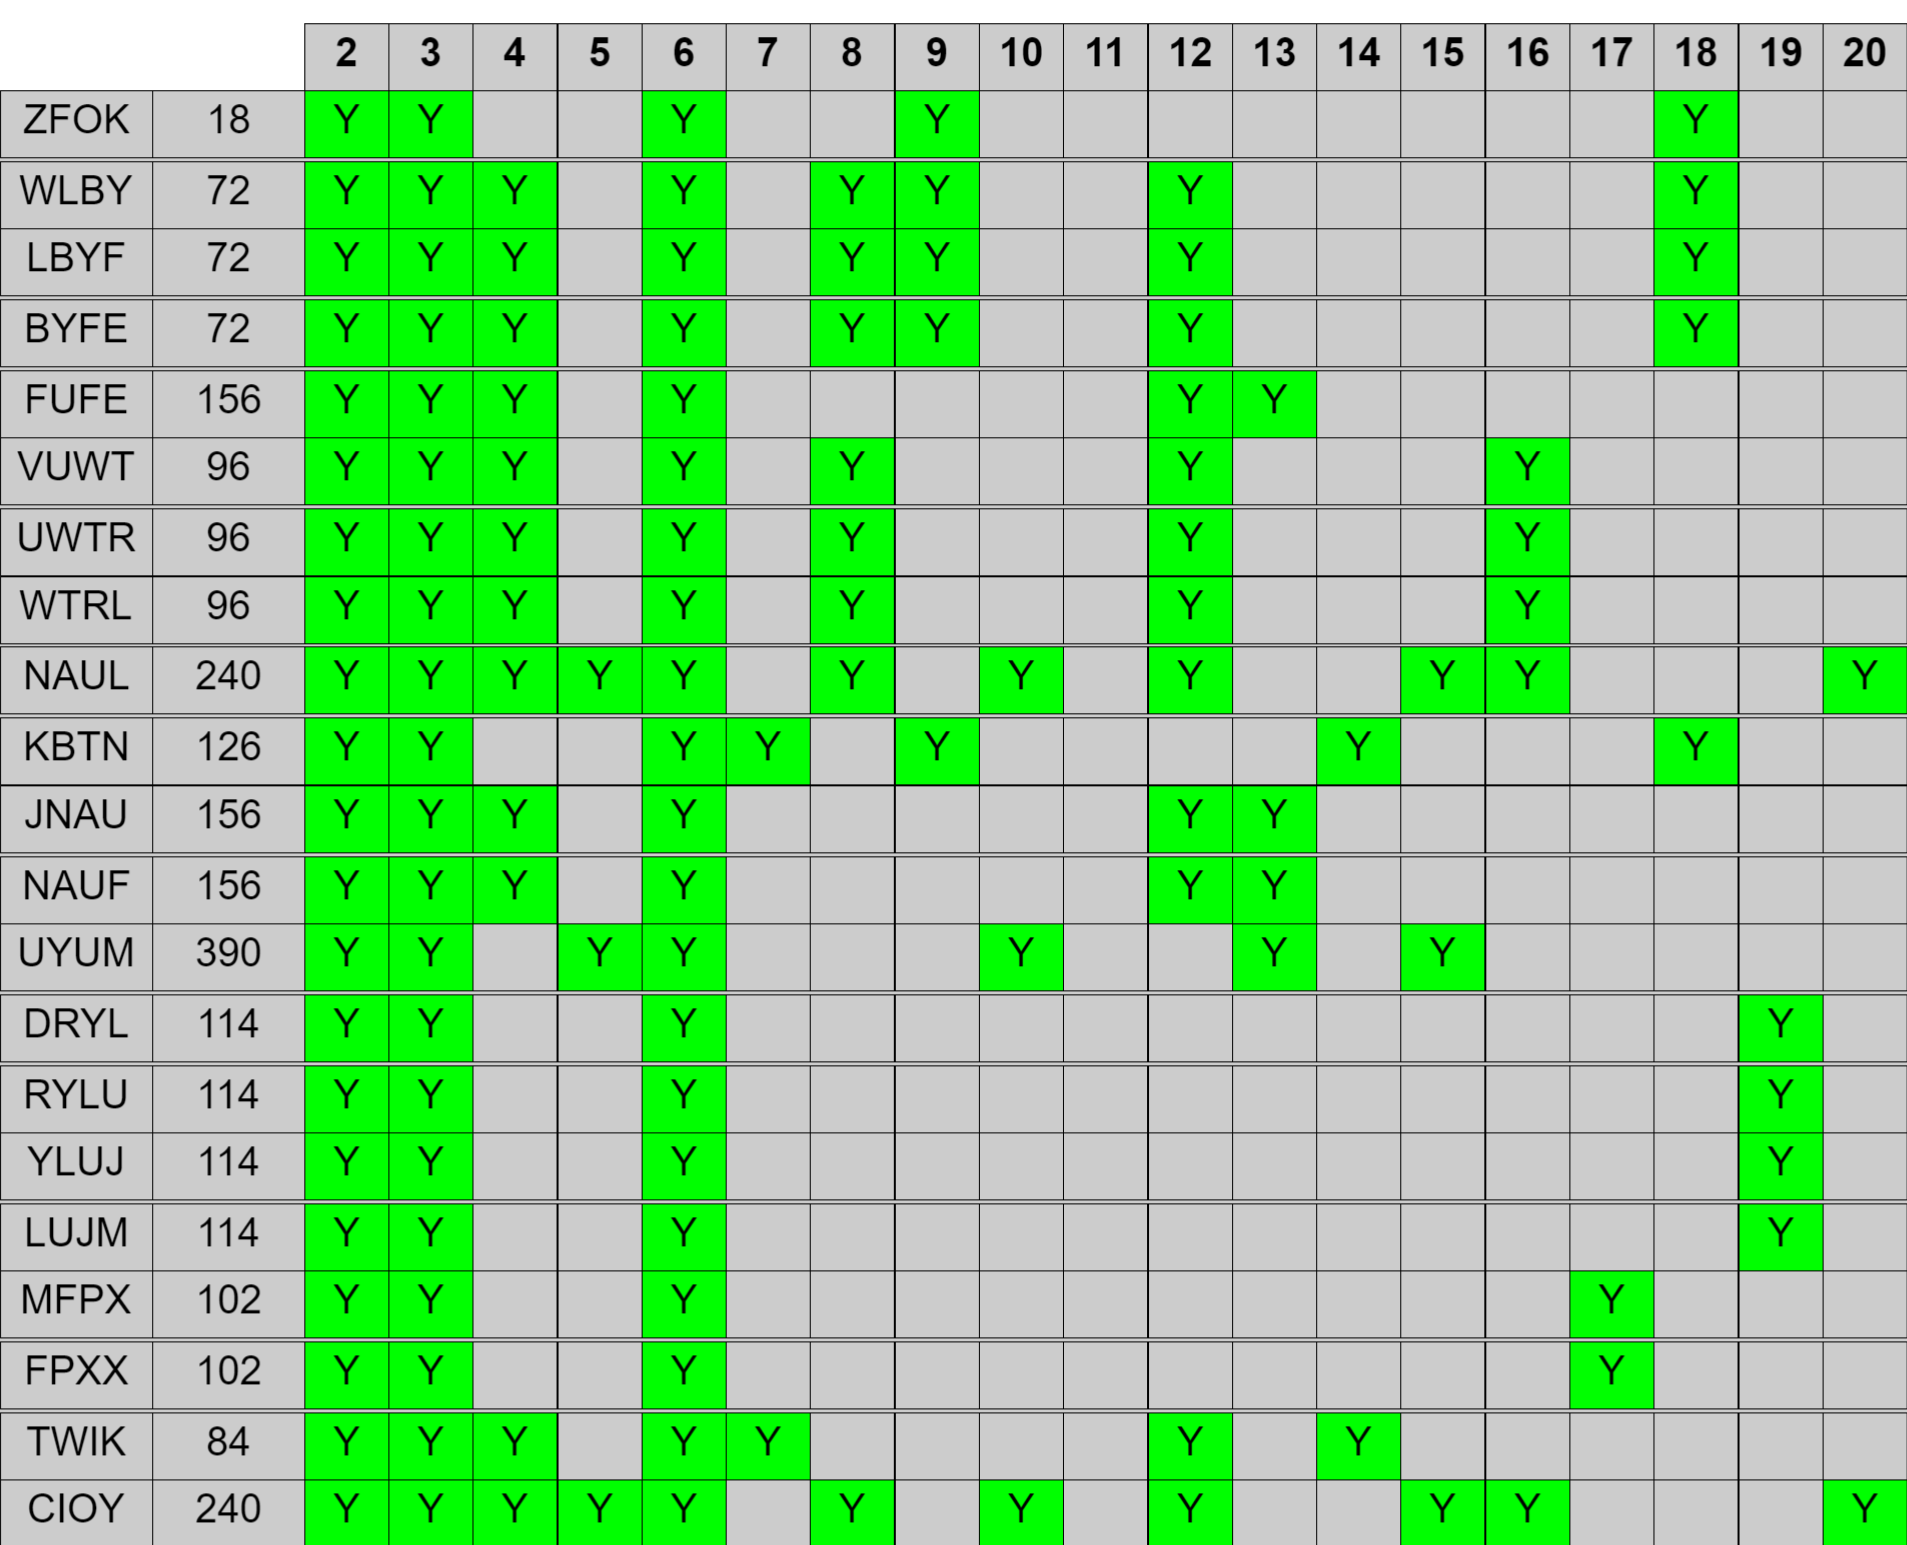
\includegraphics[scale=0.53]{repeating_strings}
\centering
\caption{}
\centering
\end{figure}
\ \\
We've successfully created a list of sets of repeating 4-graphs and 3-graphs. For each of these, we find the distance between two repeating units (the number next to the repeating unit), and then we highlight all the divisors (below 20) of this distance. So the two appearances of \textsf{ZFOK} are 18 letters apart, suggesting a keyword of length 18, 9, 6, 3 or 2.\\\\
When we look down the whole set of repeating units we are looking for the highest number that is selected in most of the pairs of repeating units. In this case, the most likely key length is 6. Notice that 2 and 3 are also very highly appearing.\\\\
It does not have to fit every single repeating unit, but there should be only few special cases that do not work; we can assume that these are purely coincidental repetitions, and can easily mislead us.\\\\
Once we are pretty sure about the length of the keyword, we can analyze each set of ciphertext letters that was encoded by the same keyword letter. In doing so, the easiest way is, with no doubt, to write the intercept out in 6 columns; we can subsequently study every column with simple frequency analysis. For example, this is frequency analysis made on L1, i.e. on the first column of the message.\\

\begin{figure}[H]
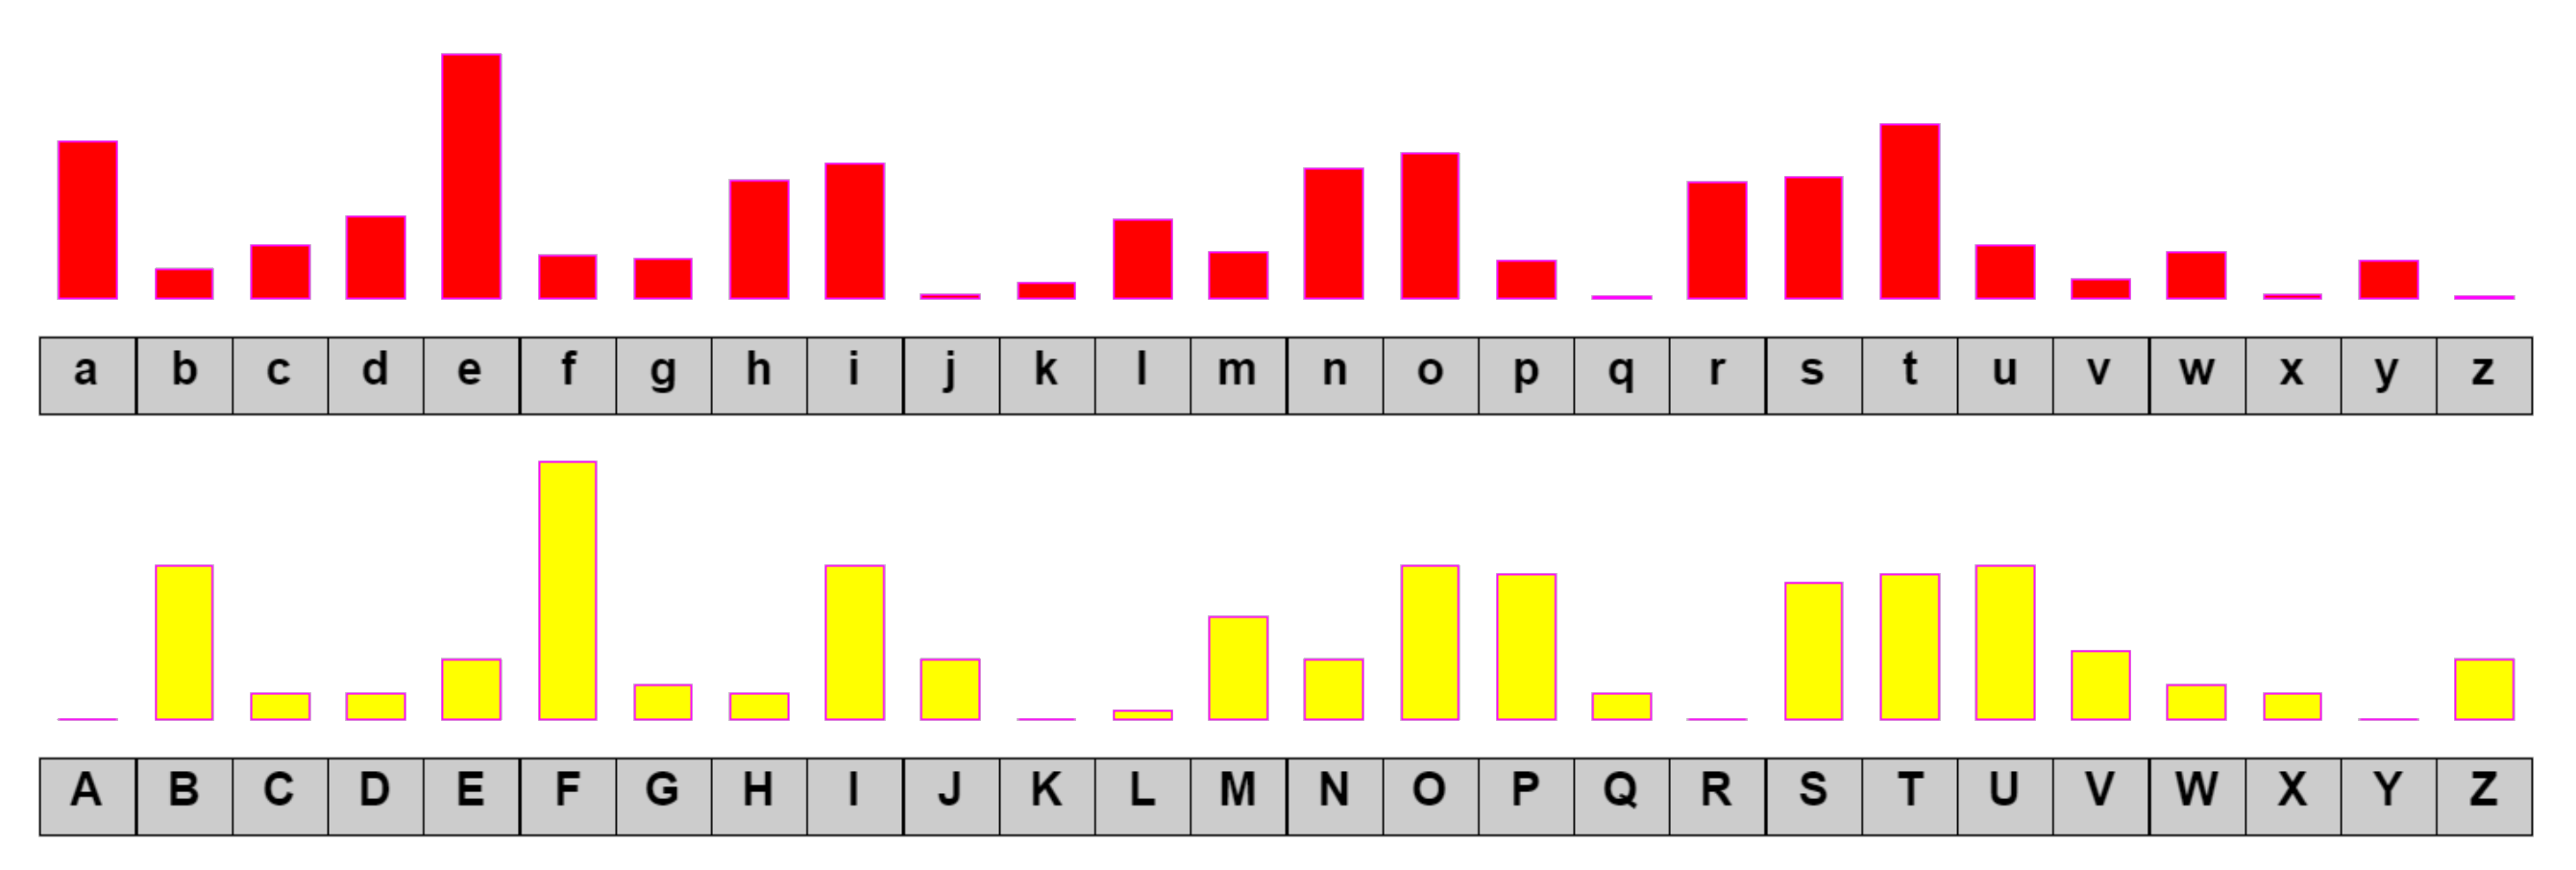
\includegraphics[scale=0.43]{kasiski_frequency_L1}
\captionsetup{justification=centering, margin=2cm}
\centering
\caption{Relative frequency of letters for the Latin alphabet (red) and for L1 (yellow). Note that L1 is right-shifted of one unity, corresponding to the letter \textsf{b}.}
\centering
\end{figure}

\ \\
After repeating this process for every level (L1,...,L6), we are able not only to recover the entire plaintext, but also the keyword (\textit{brutus}). This can happen to be very useful when more than one message is sent using the same keyword. We finally insert spaces and punctuation to retrieve the original plaintext, which is a monologue by Brutus in "Julius Caesar", written by Shakespeare.

\begin{displayquote}{\small{\textsf{Be patient till the last. Romans, countrymen, and lovers! hear me for my cause, and be silent, that you may hear: believe me for mine honour, and have respect to mine honour, that you may believe: censure me in your wisdom, and awake your senses, that you may the better judge. If there be any in this assembly, any dear friend of Caesar's, to him I say, that Brutus' love to Caesar was no less than his. If then that friend demand why Brutus rose against Caesar, this is my answer: —Not that I loved Caesar less, but that I loved Rome more. Had you rather Caesar were living and die all slaves, than that Caesar were dead, to live all free men? As Caesar loved me, I weep for him; as he was fortunate, I rejoice at it; as he was valiant, I honour him: but, as he was ambitious, I slew him. There is tears for his love; joy for his fortune; honour for his valour; and death for his ambition. Who is here so base that would be a bondman? If any, speak; for him have I offended. Who is here so rude that would not be a Roman? If any, speak; for him have I offended. Who is here so vile that will not love his country? If any, speak; for him have I offended. I pause for a reply. Then none have I offended. I have done no more to Caesar than you shall do to Brutus. The question of his death is enrolled in the Capitol; his glory not extenuated, wherein he was worthy, nor his offences enforced, for which he suffered death. Here comes his body, mourned by Mark Antony: who, though he had no hand in his death, shall receive the benefit of his dying, a place in the commonwealth; as which of you shall not? With this I depart,—that, as I slew my best lover for the good of Rome, I have the same dagger for myself, when it shall please my country to need my death.}}}
\end{displayquote}


\section{Text characterisation}
When cryptanalysing cipher, we usually try many `candidate' keys until a key is found that results in a readable output. \textbf{Text characterisation} is a way of automatically determining how close a piece of text is to natural English, which can be used as an aid to a cryptanalyst, or as a component in automatic code cracking software.
\subsection{Index of coincidence}
\textbf{Coincidence counting} is a technique, invented by William F. Friedman, of putting two texts side-by-side and counting the number of times that identical letters appear in the same position. This count, either as a ratio of the total or normalized by dividing by the expected count for a random source model, is what we call the \textit{index of coincidence}, or \textit{IC}\supercite{index_of_coincidence}.\\\\
The index of coincidence provides a measure of how likely it is to draw two matching letters by randomly selecting two letters from a given text. The chance of drawing a specific letter in the text is (number of times that letter appears / length of the text), while the chance of drawing that same letter again, without replacement, is (appearances - 1 / text length - 1). If we compute the product of these two values for any letter of the alphabet and then sum these products, we get a chance a drawing two of a kind. This probability can then be normalized by multiplying it by some coefficient $c$, typically 26 in English.\\

\begin{equation}
IC = c \times \bigg(\Big(\frac{n_{a}}{N} \times \frac{n_{a}-1}{N-1}\Big) + \Big(\frac{n_{b}}{N} \times \frac{n_{b}-1}{N-1}\Big) + ... + \Big(\frac{n_{z}}{N} \times \frac{n_{z}-1}{N-1}\Big)\bigg)
\end{equation}
\ \\
where $c$ is the normalizing coefficient, $n_a$ is the number of times the letter 'a' appears in the text, and $N$ is the length of the text.\\\\
We can express the index of coincidence for a given letter-frequency distribution as a summation:\\

\begin{equation}
IC = \frac{\sum\limits_{i=1}^{c} n_i(n_i-1)}{N(N-1)/c}
\end{equation}
\ \\
where $N$ is the length of the text and $n_1,n_2,...,n_c$ are the frequencies (as integers) of the $c$ letters of the alphabet. Note that $\sum_{i} n_i=N$ \\\\
The index of coincidence is useful both in the analysis of natural-language plaintext and in the analysis of ciphertext (cryptanalysis). Coincidence counting can help determine when two texts are written in the same language using the same alphabet. The \textit{causal} coincidence count for such texts will be distinctly higher than the \textit{accidental} coincidence count for texts in different languages, or texts using different alphabets, or gibberish texts.\\\\
In cryptanalysis, we can assume that coincidences in ciphertext are caused by coincidences in the underlying plaintext, even when only ciphertext is available for testing and plaintext letter identities are disguised.\\\\
For example, we imagine an alphabet of only the two letters \textsf{A} and \textsf{B}, and suppose that the letter \textsf{A} is used 75\% of the time, while the letter \textsf{B} 25\% of the time. If two texts in this language are laid side by side, then the following pairs can be expected:\\

\begin{center}
 \begin{tabular}{||c c||} 
 \hline
 Pair & Probability\\ [0.5ex] 
 \hline\hline
 \textsf{AA} & 56.25\% \\ 
 \hline
 \textsf{BB} & 6.25\% \\
 \hline
 \textsf{AB} & 18.75\% \\
 \hline
 \textsf{BA} & 18.75\% \\
 \hline
\end{tabular}
\end{center}
\ \\
Overall, the probability of a coincidence is 62.5\% (56.25\% + 6.25\%).\\\\
Now we consider the case then both messages are encrypted using a simple monoalphabetic substitution cipher which replaces \textsf{A} with \textsf{B} and vice versa:\\

\begin{center}
 \begin{tabular}{||c c||} 
 \hline
 Pair & Probability\\ [0.5ex] 
 \hline\hline
 \textsf{AA} & 6.25\% \\ 
 \hline
 \textsf{BB} & 56.25\% \\
 \hline
 \textsf{AB} & 18.75\% \\
 \hline
 \textsf{BA} & 18.75\% \\
 \hline
\end{tabular}
\end{center}
\ \\
The overall probability of a coincidence in this situation is 62.5\% (6.25\% + 56.25\%), exactly the same as for the unencrypted "plaintext" case. In effect, the new alphabet produced by the substitution is just a uniform renaming of the original character identities, which does not affect whether they match.\\\\
Now we suppose that only \textit{one} message (say, the second) is encrypted using the same substitution cipher $(A, B) \rightarrow (B,A)$. The following pairs can now be expected:\\

\begin{center}
 \begin{tabular}{||c c||} 
 \hline
 Pair & Probability\\ [0.5ex] 
 \hline\hline
 AA & 18.75\% \\ 
 \hline
 BB & 18.75\% \\
 \hline
 AB & 56.25\% \\
 \hline
 BA & 6.25\% \\
 \hline
\end{tabular}
\end{center}
\ \\
The probability of a coincidence in this scenario is only 37.5\% (18.75\% + 18.75\%). This is incredibly lower than the probability when same-language, same-alphabet texts were used. It's evident that coincidences are more likely when the most frequent letters in each text are the same.\\\\
The same principle applies to real languages like English, because certain letters, like \textsf{E}, occur much more frequently than other letters, so when any two English texts are compared, the coincidence count will be higher than when an English text and a foreign-language text are used.\\\\
One can think that this effect can be subtle. For example, similar languages will have a higher coincidence count than dissimilar languages. Moreover, it's not so hard to generate random text with a frequency distribution similar to real text, artificially raising the coincidence count. Nevertheless, this technique can be used effectively to identify when two texts are likely to contain meaningful information in the same language using the same alphabet, to discover periods for repeating keys, and to uncover many other kinds of nonrandom phenomena withing or among ciphertexts.\\\\
Expected values for various languages are:\\

\begin{center}
 \begin{tabular}{||c c||} 
 \hline
 Language & IC\\ [0.5ex] 
 \hline\hline
 English & 1.73 \\ 
 \hline
 French & 2.02 \\
 \hline
 Italian & 1.94 \\
 \hline
 Russian & 1.76 \\
 \hline
 Spanish & 1.94 \\
 \hline
\end{tabular}
\end{center}
\ \\

\subsubsection{Example}
As a practical illustration of the use of the index of coincidence, suppose that we have intercepted the following ciphertext message:
\begin{displayquote}{\small{\texttt{QPWKA LVRXC QZIKG RBPFA EOMFL  JMSDZ VDHXC XJYEB IMTRQ WNMEA IZRVK CVKVL XNEIC FZPZC ZZHKM  LVZVZ IZRRQ WDKEC HOSNY XXLSP
MYKVQ XJTDC IOMEE XDQVS RXLRL  KZHOV}}}
\end{displayquote}
\ \\
Suspecting this to be an English plaintext encrypted using a Vigenère cipher and a short repeating keyword, we can consider5 the ciphertext stacked into some number of columns. If the key size happens to have been the same as the assumed number of columns, then all the letters within a single column will have been enciphered using the same key letter (i.e. using a simple Caesar cipher). The corresponding set of ciphertext letters should have a roughness of frequency distribution similar to that of English. Therefore, if we compute the aggregate delta-IC for all columns, it should be around 1.73, which is the IC of natural English; on the other hand, if we have incorrectly guessed the key size (number of columns), the aggregate delta-IC should be around 1. So we compute the delta-IC for assumed key size from 1 to 10:\\

\begin{center}
 \begin{tabular}{||c c||} 
 \hline
 Key size & Delta-IC\\ [0.5ex] 
 \hline\hline
 1 & 1.12\\ 
 \hline
 2 & 1.19\\
 \hline
 3 & 1.05\\
 \hline
 4 & 1.17\\
 \hline
 5 & 1.82\\
 \hline
 6 & 0.99\\
 \hline
 7 & 1.00\\
 \hline
 8 & 1.05\\
 \hline
 9 & 1.16\\
 \hline
 10 & 2.07\\
 \hline
\end{tabular}
\end{center}
\ \\
We see that the key size is most likely five; we then stack the ciphertext into five columns and repeat the same decryption scheme we used in the example of a Kasiski examination (frequency analysis to each column). In doing so, we find the keyword \textsf{every} and the message (after inserting spaces):\\

\begin{displayquote}{\small{\textsf{Must change meeting location from bridge to underpass since enemy agents are believed to have been assigned to watch bridge stop meeting time unchanged XX}}}
\end{displayquote}
\ \\
\textsf{XX} are evidently null character used to pad out the final group for transmission. This entire procedure could easily be packaged into an automated algorithm for breaking such ciphers. Due to normal statistical fluctuation, such an algorithm will occasionally make wrong choices, especially when analyzing short ciphertext messages.

\subsection{Chi-squared test}
The \textbf{Chi-squared test}, also written $\chi^{2}$ test, is a measure of how similar two categorical probability distributions are. If the two distributions are identical, the chi-squared statistic is 0; conversely, if the distributions are very different, some higher number will result. The formula for the chi-squared statistic is:

\begin{equation}
\chi^{2}(C, E) = \sum\limits_{i=A}^{Z} \frac{(C_i - E_i)^{2}}{E_i}
\end{equation}

\ \\
where $C_A$ is the count (and not the probability) of letter \textsf{A}, and $E_A$ is the expected count of letter \textsf{A}.\\\\
In cryptanalysis, chi-squared test is used to compare the distribution of plaintext and possibly decrypted ciphertext. The lowest value of the test means that the decryption was somehow successful with high probability. This method can be generalized for solving modern cryptographic problems.\\\\

\subsubsection{Example}
If we were to try to solve a Caesar cipher by hand, a good first step would be to calculate the frequency distribution of the ciphertext characters. We could then compare them to the frequency distribution of English, and by shifting the two frequency distributions relative to one another we could find the shift that was used to encipher the plaintext.\\\\
The chi-squared statistic is a way for a computer to essentially perform this series of operations. Let's say we have a message encoded using a Caesar cipher, like this:

\begin{displayquote}{\small{\texttt{AOLJH LZHYJ PWOLY PZVUL VMAOL LHYSP LZARU VDUHU KZPTW SLZAJ PWOLY ZPAPZ HAFWL VMZBI ZAPAB APVUJ PWOLY PUDOP JOLHJ OSLAA LYPUA OLWSH PUALE APZZO PMALK HJLYA HPUUB TILYV MWSHJ LZKVD UAOLH SWOHI LAXXX}}}
\end{displayquote}
\ \\
We also know the probabilities of characters occurring in normal English text; however, the chi-squared statistic uses counts, not probabilities. As a result we need to use the probabilities to compute the expected count for each letter. For instance, if the letter \textsf{E} occurs with a probability of 0.127, we would expect it to occur 12.7 times every 100 characters. In order to calculate the expected count we just have to multiply the probability by the length of the ciphertext (162 in this case); we expect letter \textsf{E} to appear $ 162 \times 0.127 = 20.57$ times.\\\\
We then decipher the ciphertext with each of the 25 possible keys and calculate the chi-squared statistic for each one. This compares the letter counts in each decryption with what we would expect the counts to be if the text were English. In the above ciphertext, the letter \textsf{A} occurs 18 times; if it were natural English, we would expect it to appear $162 \times 0.082 = 13.284$ times. Using this information we compute the following for the letter \textsf{A}:\\

\begin{equation}
\frac{(18-13.284)^{2}}{13.284} = 1.674
\end{equation}
\ \\
We also need to perform this procedure for the other letters, then add the 26 results that we get; the result of this is around 1634.09. To find the correct key we have to do this for each key. The results are shown below:\\

\begin{center}
 \begin{tabular}{||c c||} 
 \hline
 Decryption key & $\chi^{2}$\\ [0.3ex] 
 \hline\hline
 0 & 1634.09\\
 \hline
 1 & 3441.13\\
 \hline
 2 & 2973.71\\
 \hline
 3 & 1551.67\\
 \hline
 4 & 1199.40\\
 \hline
 5 & 1466.62\\
 \hline
 6 & 1782.26\\
 \hline
 7 & \textbf{33.67}\\
 \hline
 8 & 1747.07\\
 \hline
 9 & 1386.62\\
 \hline
 10 & 3423.96\\
 \hline
 11 & 809.38\\
 \hline
 12 & 4646.96\\
 \hline
 13 & 724.11\\
 \hline
 14 & 2159.43\\
 \hline
 15 & 1787.26\\
 \hline
 16 & 3527.17\\
 \hline
 17 & 2967.66\\
 \hline
 18 & 1368.70\\
 \hline
 19 & 929.17\\
 \hline
 20 & 461.19\\
 \hline
 21 & 4395.68\\
 \hline
 22 & 703.43\\
 \hline
 23 & 1226.79\\
 \hline
 24 & 1817.85\\
 \hline
 25 & 2939.16\\
 \hline
\end{tabular}
\end{center}
\ \\
We have figured out that the key used to encipher the message was probably 7 (i.e.\ a right-shift of 7 positions), cause the chi-squared computed on that plaintext is much lower than all the others. Hence the message:

\begin{displayquote}{\small{\textsf{The Caesar cipher is one of the earliest-known and simplest ciphers. It is a type of substitution cipher in which each letter in the plaintext is shifted a certain number of places down the alphabet.}}}
\end{displayquote}

\chapter{A real-world case: the Zodiac-408 cipher}
The Zodiac was a serial killer who killed at least seven people in the late `60s and early `70s. During his killing spree, he sent a variety of messages to newspapers and police, some of which included ciphers and apparent ciphers.\\\\
The `Zodiac-408' cipher - so called because it had 408 ciphertext symbols - was a three part ciphertext, with one part sent to the \textit{Vallejo Times-Herald}, one part sent to the \textit{San Francisco Chronicle}, and the third part sent to the \textit{San Francisco Examiner}. The cipher, which is a homophonic substitution, was broken after six days of its publication by Donald and Bettye Harden, school teachers\supercite{solved_zodiac_408_cipher}.\\\\
In addition to the Zodiac-408 cipher, the Zodiac sent more messages that appear to be ciphertext: one of these, the so-called `Zodiac-340', is still unsolved. However, we will focus on the solved Zodiac-408 cipher.\\\\

\begin{figure}[H]
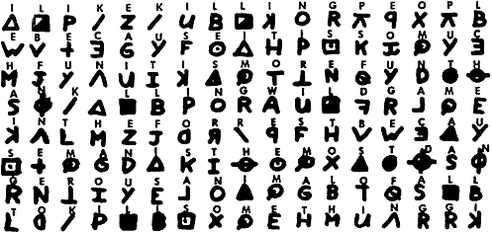
\includegraphics[scale=0.7]{zodiac_408_1}
\centering
\caption{Part 1 sent to Vallejo Times-Herald.}
\centering
\end{figure}
\ \\\\
\begin{figure}[H]
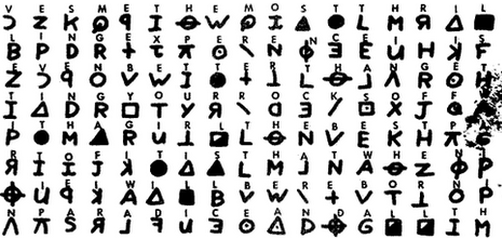
\includegraphics[scale=0.7]{zodiac_408_2}
\centering
\caption{Part 2 sent to San Francisco Chronicle.}
\centering
\end{figure}

\begin{figure}[H]
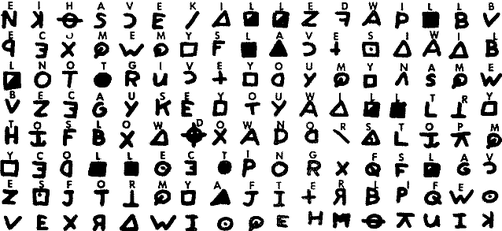
\includegraphics[scale=0.7]{zodiac_408_3}
\centering
\caption{Part 3 sent to San Francisco Examiner.}
\centering
\end{figure}
\ \\

\section{Hill Climbing}
The algorithm we'll use throughout this chapter is called \textbf{hill climbing}\supercite{homophonic_cryptanalysis}: it's an heuristic search, in the sense that it uses a series of guesses in an attempt to find a reasonable solution to a given combinatorial problem.\\\\
We'll assume that the plaintext is English: however, for a homophonic substitution cipher, multiple ciphertext symbols can represent a single plaintext. For a given homophonic cipher, let $n$ be the number of ciphertext symbols. Then we have $ n \geq 26 $ and the special case where $ n = 26 $ is a simple substitution. Furthermore, let $n_a$ be the number of ciphertext symbols that correspond to plaintext \textsf{A}, let $n_b$ be the number of symbols that correspond to \textsf{B}, and so on. Then:\\

\begin{equation}
n_a + n_b + n_c + ... + n_z = n
\end{equation}
\ \\
Our algorithm consists of the following three `layers':
\begin{itemize}
\item Inner hill climb layer
\item Random initial key layer
\item Outer hill climb layer
\end{itemize}
\ \\
In the outer hill climb, we determine values $n_a, n_b, ..., n_z$ subject to the constraint that $n_a + n_b + ... + n_z = n$. Then in the random key layer, we generate multiple random initial keys, subject to the constraint from the outer hill climb layer. Finally, for the inner hill climb we build up several putative keys and define a score for each of them.\\\\

\begin{figure}[H]
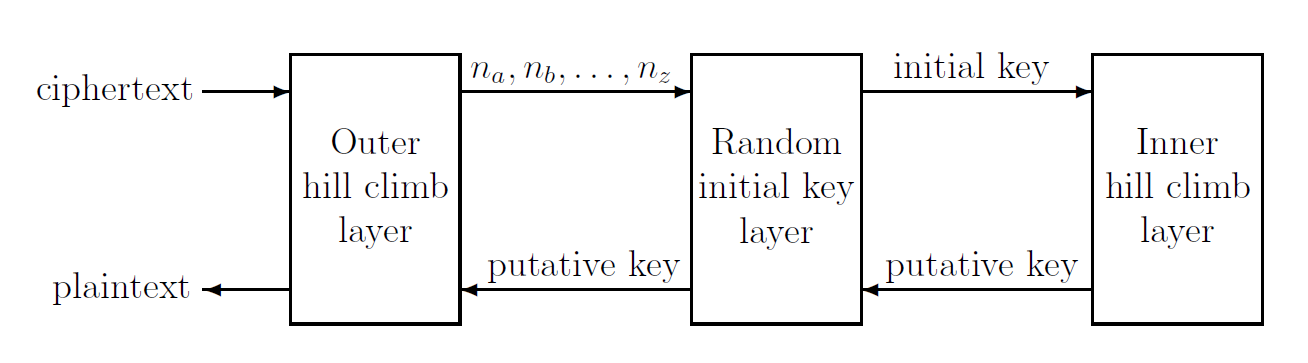
\includegraphics[scale=0.35]{hill_climb_scheme}
\centering
\caption{}
\centering
\end{figure}
\ \\

\subsection{Inner Hill Climb Layer}
We first note that any solution at this phase is subject to the constraint that $n_a$ ciphertext symbols map to \textsf{A}, $n_b$ symbols map to \textsf{B}, and so on. That is, the values of $n_a, n_b, ..., n_z$ do not change at this layer. We also have an initial key, which is generated in the random key layer.\\
\subsubsection{Modify the putative key}
We modify the putative key by swapping elements, as follows. First, denote the putative key as $K = (k_1, k_2, ..., k_n)$, where $K$, supposing that we have the particular case $n=26$, is a permutation of the 26 English letters. The swapping will be done systematically through a series of rounds. In the first round, all adjacent elements are selected for swapping, that is, $k_1$ is swapped with $k_2$, then $k_2$ is swapped with $k_3$, and so on. In the second round, the elements in $K$ at distance two are swapped, while in the third round, elements at distance of three are swapped, and so on.\\\\
However, letters can appear multiple times in the key and we must avoid swapping a letter with itself - swapping a letter with itself would not change the putative plaintext. The number of swaps required depends on $n$ and the values $n_a, n_b, ..., n_z$. Let $m_i$, for $i=1,2,...,26$ be the values of $n_a, n_b, ..., n_z$ respectively. Then each of $m_1$ identical letters is swapped with all $n-m_1$ other letters, each of the $m_2$ identical letters is swapped with all remaining $n - m_1 - m_2$ letters and so on. Thus, the total number of swaps is given by:\\

\begin{equation}
\sum_{i=1}^{26} m_i(n-\sum_{j=1}^{i} m_j) = \sum_{i=1}^{25} \sum_{j=i+1}^{26} m_i m_j
\end{equation}
\ \\\\
In practice, we consider all ${n}\choose{2}$ pairs of ciphertext symbols, and we simply skip any pairs that currently map to the same plaintext letter. Consequently, a crude upper bound on the number of swaps is given by ${n}\choose{2}$.\\

\subsubsection{Compute the score}
First of all, we have to fill out a $ 26 \times 26 $ matrix $E$ which contains expected digram frequencies for English: this can be easily found on statistics websites. Every cell of this matrix, say the first, `aa', gives us the percentage of that particular digram in a normal English text. For example, the digram \textsf{th} is the most frequent one.\\\\
\begin{figure}[H]
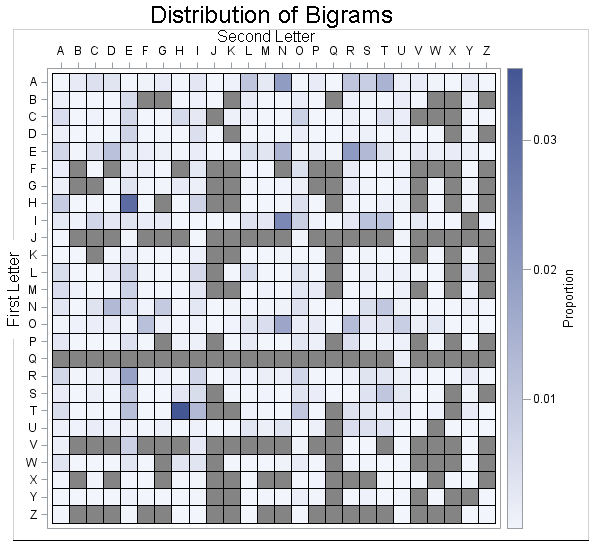
\includegraphics[scale=0.6]{digramfreqmatrix}
\centering
\caption{}
\centering
\end{figure}
\ \\
Moreover, let $D_C$ be a $n \times n$ matrix containing ciphertext digram frequencies. This matrix, which is constructed only once, and never changes, is used as a `rosetta stone' to translate digrams of the ciphertext into digrams of standard English, using the current putative key. In this way, we construct a second matrix $D_P$, of size $26 \times 26$, which we can use to compare to $E$: this matrix contains the letter digram frequencies corresponding to the current putative plaintext. Obviously, this matrix has to change whenever our current putative key is modified.\\\\
Once we have determined $D_P$, the score computation is done in this way:\\

\begin{equation}
score{(K)} = d{(D_P, E)} = \sum_{i,j} |d_{ij} - e_{ij}|
\end{equation}
\ \\\\
Note that $score \geq 0$, with $score = 0$ being a perfect match, and the smaller the score, the better the key $K$. If the new score computed is less than the current better score, we update its value to the new score and change the current putative key with the new $K$.\\ 
\begin{algorithm}[H]
	$innerScore = d(D_p, E)$\\
	\For{$i=1 \ to\  n-1$}
	{
		\For{$j=1 \ to\ n-i$}
		{
			$K' = K$\\
			$swap(k'_j, k'_{j+1})$\\
			$D' = \text{digram matrix for } K' \text{ using } D_p \text{ and } D_c$\\
			\If{$d(D', E) < innerScore$}
			{
				$innerScore = d(D', E)$\\
				$K = K'$\\
				$D_p = D'$\\
			}
		}
	}
	\Return $innerScore$
	\caption{Inner Hill Climb}
\end{algorithm}
\ \\
\subsection{Random Initial Key Layer}
Choosing an optimal initial key could be very complicated, so we use a simple greedy approach. Specifically, we find subsets that approximate the letter frequencies, beginning with the highest-frequency letters and proceeding to the lower-frequency letters. That is, we first find a subset of size $n_e$ that is a reasonable approximation to the expected frequency of \textsf{E}, followed by a subset of size $n_t$ that approximates the expected frequency of \textsf{T}, followed by a subset of size $n_a$ that approximates the frequency of \textsf{A} in English text, and so on.\\\\
For example, suppose that $n_e = n_t = 2$ and $n_a = 1$, and we have the following ciphertext frequencies:
\begin{figure}[H]
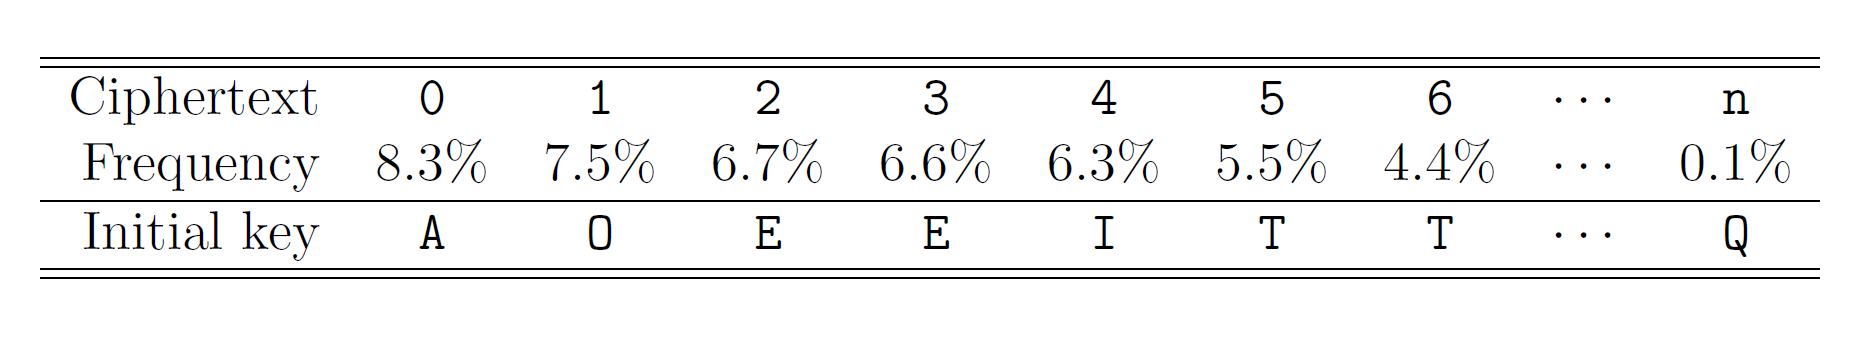
\includegraphics[scale=0.27]{random_key_layer}
\centering
\caption{}
\centering
\end{figure}
\ \\
We see that ciphertext symbols \textsf{4} and \textsf{5} can be combined to give a good approximation (12.9\%) to the expected frequency of plaintext letter \textsf{E} (12.7\%). Similarly, symbols \textsf{6} and \textsf{7} together approximate the expected frequency of \textsf{T} while symbol \textsf{1} approximates the expected frequency of \textsf{A}.\\\\
Note that this approach will generally find good approximations for the higher frequency letters, but may not be as accurate for the lower frequencies letters. This is a reasonable compromise between efficiency and accuracy, since the high frequency letters will have the largest impact on the solution.\\\\
One way to improve the results of this layer is to conduct the attack multiple times using different initial starting points: therefore, we generate $R$ distinct initial keys. For each of the $R$ iterations, we select a subset of $n_e$ ciphertext symbols that map to \textsf{E}, and $n_t$ ciphertext symbols that map to \textsf{T}, and so on.\\\\
For each of the $R$ initial putative keys generated at this layer, we first determine the corresponding $D_p$, then complete the inner hill climb. The final result of the random initial key layer is the best-scoring putative key obtained in any of these $R$ iterations over the inner hill climb.\\

\begin{algorithm}
	$(n_a, n_b,..., n_z) \gets \text{provided by the outer hill climb layer}$\\
	$bestInitScore = \infty$\\
	\For{$r=1 \ to\ R$}
	{
		$\text{randomly initialize } K = (k_1, k_2,..., k_n) \text{ satisfying } n_a, n_b, ..., n_z$\\
		$D_p = \text{digram matrix from } D_c \text{ and } K$\\
		$initScore = InnerHillClimb(D_p)$\\
		\If{$initScore < bestInitScore$}
		{
			$bestInitScore = initScore$\\
			$bestInitKey = K$\\
		}
	}
	\Return $bestInitScore$
	\caption{Random Initial Key}
\end{algorithm}

\subsection{Outer Hill Climb Layer}
The outer hill climb layer specifies the number of ciphertext symbols that are mapped to each letter. We initially specify $n_a, n_b, ..., n_z$ with $n_a + n_b + ... + n_z = n$, then we iterate, where at each iteration we modify these subset sizes by `swapping' adjacent pairs (ranked from high to low frequency).\\\\
First, we need to specify an initial distribution to begin the outer hill climb: we assume that the mapping of letters to ciphertext symbols was chosen to flatten the ciphertext statistics as much as possible. That is, we assume that about 12\% of the symbols correspond to \textsf{E}, while the letter \textsf{T} corresponds to about 9\% of the symbols, and so on. We also assume that at least one symbol corresponds to each letter of the alphabet.\\\\
Now we have to describe the `swapping' process in more detail: suppose we have $n=35$, which gives us for example $n_e = 4$ and $n_t = 2$. Using these values, we first execute the random initial key layer which, in turn, calls the inner hill climb. The best score of this entire process is saved as the current $score$. Then we apply our `swap', starting with $n_e$ and $n_t$. However, instead of simply swapping the values, we increment $n_e$ and decrement $n_t$. So, for this example, the first swap consists of setting $n_e = 5$ and $n_t = 1$, with the remaining values unchanged. Using the new distribution, we call the random initial key layer, and if the best score from this process is less than $score$, then we update $score$ and maintain this new distribution; otherwise, $score$ remains unchanged and we revert to the previous distribution.\\\\
If the score does not improve, then we switch the order of the pair: for the example above, we would increment the original $n_t$ and decrement the original $n_e$. Like in the inner hill climb layer, we perform the swap on all consecutive pairs, then on all pairs at distance 2, then all pairs at distance 3, and so on.\\

\begin{algorithm}
	$K = bestInitKey = bestKey = \text{NULL}$\\
	$\text{parse ciphertext to determine } D_c$\\
	$\text{initialize } n_a, n_b, ..., n_z \text{ as described above}$\\
	$(m_1, m_2, ..., m_{26}) = (n_a, n_b, ..., n_z)$\\
	$bestScore = RandomInitialKey(m_1, m_2, ..., m_{26})$\\
	$bestKey = bestInitKey$\\
	\For{$i=1\ to \ 25$}
	{
		\For{$j=1 \ to \ 26-i$}
		{
			$(m'_1, m'_2, ..., m'_{26}) = (m_1, m_2, ..., m_{26})$\\
			$increment(m'_j)$\\
			$decrement(m'_{j+1})$\\
			$score = RandomInitialKey(m'_1, m'_2, ..., m'_{26})$\\
			\uIf{$score < bestScore$}
			{
				$(m_1, m_2, ..., m_{26}) = (m'_1, m'_2, ..., m'_{26})$\\
				$bestScore = score$\\
				$bestKey = bestInitKey$\\
			}
			\Else
			{
				$(m'_1, m'_2, ..., m'_{26}) = (m_1, m_2, ..., m_{26})$\\
				$increment(m'_{j+1})$\\
				$decrement(m'_j)$\\
				$score = RandomInitialKey(m'_1, m'_2, ..., m'_{26})$\\
				\If{$score < bestScore$}
				{
					$(m_1, m_2, ..., m_{26}) = (m'_1, m'_2, ..., m'_{26})$\\
					$bestScore = score$\\
					$bestKey = bestInitKey$\\
				}
			}
		}	
	}
	\Return $bestKey$
	\caption{Outer Hill Climb}
\end{algorithm}

% The [1] after the \footnote command is a number indicating to use asterisk instead of numbers
% See the footmisc package
\section{Results}
In order to attack the cipher, we used a C++ code\supercite{homophonicattackcode} written by Amrapali Dhavare\footnote[1]{San Jose State University, department of Computer Science} and Markus Amalthea Magnuson, as it fully implements the algorithm described above. We made partial modifications to the code in order to adapt it to our case scenario.\\\\
Instead of using a standard $E$ matrix equivalent to the English digram frequencies, we used another matrix whose elements were the average between the standard English digram frequencies and the frequency of the same digrams in messages we know for sure were written by the Zodiac killer. For example, if the digram \textsf{wh} never appeared in the Zodiac messages, his frequency would be a half of that of standard English.\\\\
We ran a loop of 4 instances of the program for a total runtime of about 96h; the CPU we used was the \textsf{Intel i5-6600} (4 cores, 4 threads), and our UNIX-like environment was \textbf{Arch Linux}. We saved the result with the minimum score in a text file.\\\\
However, we had to make some manual adjustments to retrieve the correct solution. For example, the putative plaintext we came up with for the first message (the one sent to Vallejo Times-Herald) was this:\\

\begin{displayquote}\texttt{alokekellingpiopl\\
etecauseamossomuc\\
cfunetismoqebunth\\
adkallongweldgame\\
intceforrifmtecau\\
semanasihemottdan\\
geqoueanamaloball\\
tokollsomemcenggi\\
}
\end{displayquote}
\ \\
We can easily identify some common misspelled English words: \texttt{kelling} in the first line probably stands for \textsf{killing}, \texttt{tecause} - which appears twice in the excerpt - can lead us to think it's \textsf{because}, the expression \texttt{somuccfun} could be the equivalent of \textsf{so much fun}, \texttt{weldgame} possibly replaces the correct \textsf{wild game}, and so on.\\\\
By repeating this scheme over and over, we can rapidly find out how each ciphertext symbol maps to a letter of the English alphabet; thus, we are able to reconstruct the entire message. Moreover, it should become easier as far as we progressively decode more symbols.\\

\begin{figure}[H]
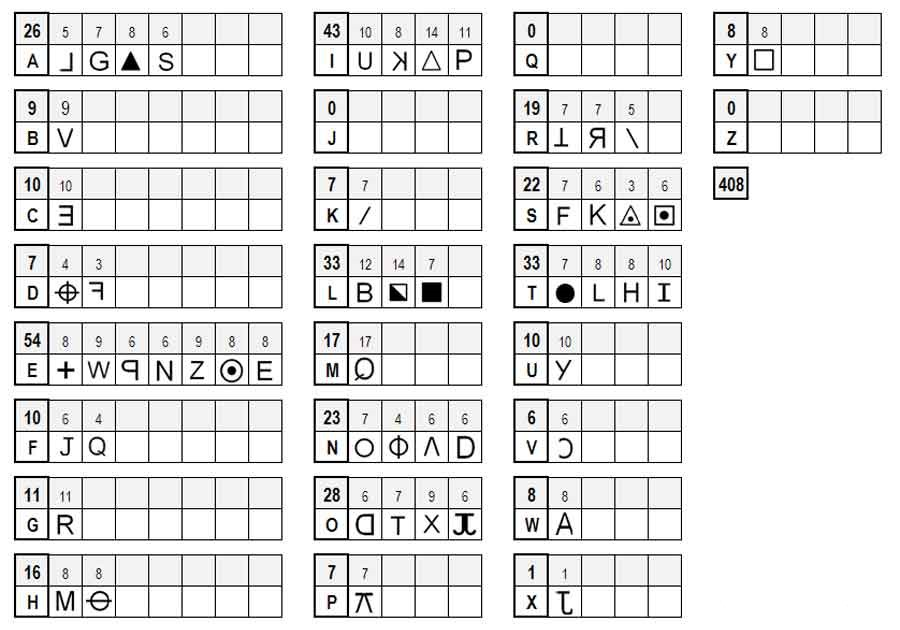
\includegraphics[scale=0.55]{zodiac_408_mapping}
\centering
\caption{Solution of the Zodiac-408 cipher.}
\centering
\end{figure}
\ \\
Once we're done with this tedious manual work (which, nonetheless, can also be automated), we finally recover the plaintext of the infamous Zodiac-408 cipher:\\
\begin{displayquote}{\small{\textsf{I like killing people because it is so much fun it is more fun than killing wild game in the forrest because man is the most dangerous animal of all to kill something gives me the most thrilling experience it is even better than getting your rocks off with a girl the best part of it is that when I die I will be reborn in paradise and all thei have killed will become my slaves I will not give you my name because you will try to slow down or atop my collection of slaves for my afterlife. Ebeorietemethhpiti.}}}
\end{displayquote}

\chapter*{Conclusions}
\addcontentsline{toc}{chapter}{Conclusions}
We discussed substitution ciphers and their security in detail.

The introduction chapter gave us the opportunity to discuss the main aspects of cryptography and why we need it (and needed it in the past), so we described how it can assure us confidentiality about the information we're dealing with.

The second, third and fourth chapter focused on the principal classes of substitution ciphers (monoalphabetic, polyalphabetic, homophonic, polygraphic) while still discussing the possible security flaws for each of them.

In the last two chapters, we showed standard techniques along another approach called hill climb (a little more sophisticated), which can be used to successfully attack substitution ciphers: all of them use statistical measures which describe how the putative plaintext we come up with is `close' to natural English.

We then applied the hill climb algorithm to a real-world case, i.e.\ one of the infamous Zodiac ciphers, and we found out a decent solution based on digrams frequencies, which still requires some manual adjustments to retrieve the correct plaintext. It might seem natural to try to extend the scoring to include, say, trigrams, but the work factor of the algorithm would increase exponentially. Another potential modification would be to include a word specified by the user which they think might appear in the plaintext, and this word can be tried at every offset in the ciphertext.

Various heuristic search techniques could be combined with the general approach: for example, the outer hill climb layer could be replaced by a genetic algorithm\supercite{geneticalgorithm}, which can generate high-quality solutions to the problem of improving the putative plaintext.

\begin{appendices}
\chapter{Transposition ciphers}
The other big family of classical ciphers is the one of transpositions ciphers: these methods of encryption rely their security on the fact that the ciphertext consitutes a permutation of the plaintext. That is, the order of the symbols (or group of symbols) is changed, in particular shifted according to a regular system.

\section{Rail fence cipher}
The rail fence cipher (also known as zigzag cipher) is one of the simplest form of transposition cipher; it derives its name from the way in which it is encoded.\\\\
In this cipher, the plaintext is written downwards and diagonally on successive `rails` of an imaginary fence, then moving up when the bottom has been reached. When we reach the top rail, the message is written downwards again until the whole plaintext is written out. The message is then read off in rows.\\\\
In this example, we have 3 rails and our message is `\textsf{WE ARE DISCOVERED, FLEE AT ONCE}':\\\\

\begin{figure}[H]
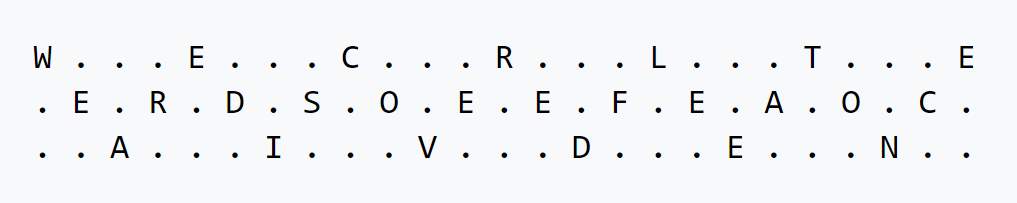
\includegraphics[scale=0.42]{rail_fence}
\centering
\caption{}
\centering
\end{figure}
\ \\
Then we read off to get the ciphertext: \colorbox{gray!12}{\small{\texttt{WECRLTEERDSOEEFEAOCAIVDEN}}}\\\\

\section{Route cipher}
In a route cipher, the plaintext is first written out in a grid of given dimensions, then read off in a pattern given in the key. For example, using the same message used in the rail fence example:\\\\
\begin{figure}[H]
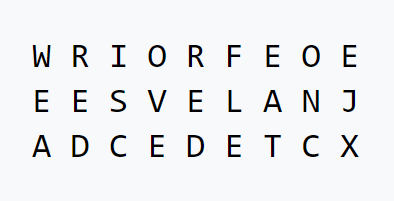
\includegraphics[scale=0.42]{route}
\centering
\caption{}
\centering
\end{figure}
\ \\
The key might specify `spiral inwards, clockwise, starting from the top right', which would give a ciphertext of \colorbox{gray!12}{\small{\texttt{EJXCTEDECDAEWRIORFEONALEVSE}}}.\\\\
Route ciphers have many more keys than a rail fence: in fact, for messages of reasonable length, the number of possible keys is potentially so huge that it cannot be enumerated even by modern computers. However, not all keys are equally good, because badly chosen routes will leave excessive chunks of plaintext, or text simply reversed, which would give cryptanalysts a nice clue on how the route has been chosen.\\\\

\section{Columnar transposition}
In a columnar transposition cipher, the plaintext is written out in rows of a fixed length, and then read out again column by column, and the columns are chosen in some scrambled order. Both the width of the rows and the permutation of the columns are often defined by a keyword.\\\\For example, the keyword \textsf{ZEBRAS} has length 6 (length of the rows), and the permutation is defined by the alphabetical order of the letters in the keyword, which in this case is 6, 3, 2, 4, 1, 5. Any spare spaces are usually filled with nulls (random characters). If the message is the same as before, we fill out this grid:\\\\

\begin{figure}[H]
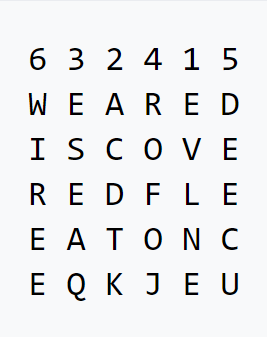
\includegraphics[scale=0.42]{columnar_regular}
\centering
\caption{}
\centering
\end{figure}
\ \\
We provided five nulls (\textsf{QKJEU}), which can be selected randomly as they are just not part of the original message.\\\\
The ciphertext then read off as: \colorbox{gray!12}{\small{\texttt{EVLNE ACDTK ESEAQ ROFOJ DEECU WIREE}}}.\\\\
A variant (called \textit{irregular}), does not make use of nulls, but the spaces are left blank: so in the example above, the grid would be filled out like this:\\\\

\begin{figure}[H]
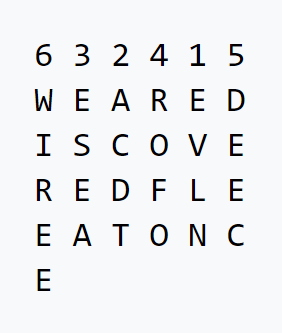
\includegraphics[scale=0.42]{columnar_irregular}
\centering
\caption{}
\centering
\end{figure}
\ \\
This would result in the ciphertext: \colorbox{gray!12}{\small{\texttt{EVLNA CDTES EAROF ODEEC WIREE}}}.\\\\

\section{Double columnar transposition}
A single columnar transposition could be attacked by guessing possible column lengths, writing the message out it its columns (but in the wrong order, as the key is not yet known), and then looking for possible anagrams of known words. Thus to make it stronger, a double transposition was often used in the past; this is simply a columnar transposition applied twice. The same key can be used for both transpositions, or two different keys can be used.\\\\
For instance, we can take the result of the irregular columnar transposition in the previous section, and perform a second encryption with a different keyword, \textsf{STRIPE}, which gives the permutation 5, 6, 4, 2, 3, 1.\\\\

\begin{figure}[H]
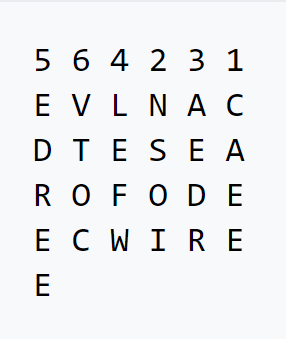
\includegraphics[scale=0.42]{double_columnar}
\centering
\caption{}
\centering
\end{figure}
\ \\
As before, this is read off columnwise to get the ciphertext: \par\colorbox{gray!12}{\small{\texttt{CAEEN SOIAE DRLEF WEDRE EVTOC}}}.\\\\

\section{Detection and cryptanalysis}
Transposition ciphers do not affect the frequency of individual symbols, so they can be easily detected by the cryptanalyst by doing a frequency count. They can surely be attacked by anagramming - sliding pieces of ciphertext around, then looking for sections that look like anagrams of English words, and solving the anagrams. Once such anagrams have been found, they reveal information about the transposition pattern, and can consequently be extended.\\\\
For these reasons, transposition is often combined with a substitution cipher, resulting in a cipher that avoids the weaknesses of both. In fact, replacing high frequency ciphertext symbols with high frequency plaintext letters does not reveal chunks of plaintext because of the transposition, and anagramming the transposition does not work because of the substitution.
\end{appendices}	

\backmatter
% bibliography
% \cleardoublepage
% \phantomsection

% Remember to run Biber first!
\printbibliography[title=References,heading=bibintoc]

% \bibliographystyle{unsrt} % BibTeX style
% \bibliography{bibliography} % BibTeX database without .bib extension

\end{document}
